%
\chapter{The One And Only}
\minitoc \onehalfspace%
Here you can place a quick introduction to the chapter; no more than a paragraph. It should put the chapter into context in terms of the rest of the thesis. In the case of including unmodified journal articles in your thesis, you can put the manuscript abstract here instead. The `\verb+\minitoc+' command prints the relevant subset of the Table of Contents at the beginning of each individual chapter.
%
%
%
%==============================================================================
\section{Introduction}
%
Welcome to \LaTeX!\footnote{Note that \LaTeX~is actually pronounced `lah-tech'. If you pronounce it as `lay-teks', anyone who knows what they're talking about will know you don't.} Here I will try to describe the basics of document creation and editing, how to use this template, etc.. Hopefully this will inspire you to stop procrastinating and start writing your thesis~\cite{upper1974}, make the writing process more efficient, and give you an attractive-looking document once it's all done.

\LaTeX~is a `document markup language'. Although programs like Word allow you to edit a document exactly as it appears in print, this can be detrimental for complex or large documents; for instance, when you insert a sentence into the document and it ruins the placement of every single figure subsequent to that insertion. In \LaTeX, you provide the contents of the document in plain text, and use commands to control how you want the document to appear; it is then {\em compiled} into a printable document. It disentangles the {\em content} and the {\em formatting} of the document, so that one can be changed without substantially affecting the other.

This PDF document was compiled from the \verb+.tex+ files provided in the template. The first step in making use of this template is getting to the point where you can re-generate this document yourself from the underlying \verb+.tex+ files. Once you can do this, you can begin inserting your own content to turn it into a thesis.
%
%
\section{Installation \& compilation}
%
First, you need the necessary programs that will interpret the \LaTeX~code and generate the output document. If you are running Linux, install the necessary TexLive packages using whatever package manager you are using (if you run into problems compiling the template, you're probably missing one of these packages). If you're a Windows user, install MiK\TeX~(\verb+miktex.org+).

Next, you'll need a text editor for making changes to the \verb+.tex+ files. Do \underline{not} use a document editor such as Word to edit these files; it may add its own formatting and corrupt them! Any program that allows you to modify plain text is OK, but I would recommend downloading and installing a program called TexMaker; it's designed specifically for creating documents using \LaTeX, is available for all platforms, and comes with all sorts of handy features.

Now it's time to see if everything is set up correctly. If you're running Linux, you can run the \verb+build+ script provided in the template from a Bash terminal. If using TexMaker, open the file \verb+thesis.tex+, and press the arrow button to the left of ``Quick Build''. Hopefully this will re-generate the file `\verb+thesis.pdf+'.

If it doesn't work, you'll need to do some debugging. Unfortunately I can't cover every single possible problem here, so make Google your friend. However one I encountered when trying to get this working on Windows was that TexMaker would give a ``Could not start the command'' message when trying to compile; if this happens, go to ``Options'' $\rightarrow$ ``Configure Texmaker'', and in the entries for PdfLaTeX and Bib(la)tex, replace the command names with the full paths to the executables (if you did a default install, they will be in \verb+C:/Program Files/MiKTeX 2.9/miktex/bin/x64/+ or something similar).

If you don't use the \verb+build+ script provided, you may find that sometimes you make changes to your thesis, re-compile the document, but not everything is updated accordingly in the PDF (e.g. table of contents). This is just a weird quirk of \LaTeX. If you re-compile again, everything that didn't update should fix itself. Updating bibliography citations is however a separate problem; see Section~\ref{la_citations} for more details on this.
%
%
\section{Document structure \& expansion}
\label{la_structure}
%
The ``master document'' of the template is the file \verb+thesis.tex+. This file is responsible for loading the necessary \LaTeX~styles and whatnot, adding the necessary thesis content before the start of the chapters, and then adding chapters to the document one by one. By default, the document will be created in a two-page format, with extra margin on the left side of odd pages and the right side of even pages (to account for the binding).

All of the stuff prior to the thesis chapters (acknowledgments, preface etc.) are loaded in the order specified by the University of Melbourne. So they shouldn't be moved around at all; you just need to add your own content to the relevant \verb+.tex+ files.

This template contains a single thesis chapter --- \verb+ch-1.tex+. It is inserted into the document by the command `\verb+%
\chapter{The One And Only}
\minitoc \onehalfspace%
Here you can place a quick introduction to the chapter; no more than a paragraph. It should put the chapter into context in terms of the rest of the thesis. In the case of including unmodified journal articles in your thesis, you can put the manuscript abstract here instead. The `\verb+\minitoc+' command prints the relevant subset of the Table of Contents at the beginning of each individual chapter.
%
%
%
%==============================================================================
\section{Introduction}
%
Welcome to \LaTeX!\footnote{Note that \LaTeX~is actually pronounced `lah-tech'. If you pronounce it as `lay-teks', anyone who knows what they're talking about will know you don't.} Here I will try to describe the basics of document creation and editing, how to use this template, etc.. Hopefully this will inspire you to stop procrastinating and start writing your thesis~\cite{upper1974}, make the writing process more efficient, and give you an attractive-looking document once it's all done.

\LaTeX~is a `document markup language'. Although programs like Word allow you to edit a document exactly as it appears in print, this can be detrimental for complex or large documents; for instance, when you insert a sentence into the document and it ruins the placement of every single figure subsequent to that insertion. In \LaTeX, you provide the contents of the document in plain text, and use commands to control how you want the document to appear; it is then {\em compiled} into a printable document. It disentangles the {\em content} and the {\em formatting} of the document, so that one can be changed without substantially affecting the other.

This PDF document was compiled from the \verb+.tex+ files provided in the template. The first step in making use of this template is getting to the point where you can re-generate this document yourself from the underlying \verb+.tex+ files. Once you can do this, you can begin inserting your own content to turn it into a thesis.
%
%
\section{Installation \& compilation}
%
First, you need the necessary programs that will interpret the \LaTeX~code and generate the output document. If you are running Linux, install the necessary TexLive packages using whatever package manager you are using (if you run into problems compiling the template, you're probably missing one of these packages). If you're a Windows user, install MiK\TeX~(\verb+miktex.org+).

Next, you'll need a text editor for making changes to the \verb+.tex+ files. Do \underline{not} use a document editor such as Word to edit these files; it may add its own formatting and corrupt them! Any program that allows you to modify plain text is OK, but I would recommend downloading and installing a program called TexMaker; it's designed specifically for creating documents using \LaTeX, is available for all platforms, and comes with all sorts of handy features.

Now it's time to see if everything is set up correctly. If you're running Linux, you can run the \verb+build+ script provided in the template from a Bash terminal. If using TexMaker, open the file \verb+thesis.tex+, and press the arrow button to the left of ``Quick Build''. Hopefully this will re-generate the file `\verb+thesis.pdf+'.

If it doesn't work, you'll need to do some debugging. Unfortunately I can't cover every single possible problem here, so make Google your friend. However one I encountered when trying to get this working on Windows was that TexMaker would give a ``Could not start the command'' message when trying to compile; if this happens, go to ``Options'' $\rightarrow$ ``Configure Texmaker'', and in the entries for PdfLaTeX and Bib(la)tex, replace the command names with the full paths to the executables (if you did a default install, they will be in \verb+C:/Program Files/MiKTeX 2.9/miktex/bin/x64/+ or something similar).

If you don't use the \verb+build+ script provided, you may find that sometimes you make changes to your thesis, re-compile the document, but not everything is updated accordingly in the PDF (e.g. table of contents). This is just a weird quirk of \LaTeX. If you re-compile again, everything that didn't update should fix itself. Updating bibliography citations is however a separate problem; see Section~\ref{la_citations} for more details on this.
%
%
\section{Document structure \& expansion}
\label{la_structure}
%
The ``master document'' of the template is the file \verb+thesis.tex+. This file is responsible for loading the necessary \LaTeX~styles and whatnot, adding the necessary thesis content before the start of the chapters, and then adding chapters to the document one by one. By default, the document will be created in a two-page format, with extra margin on the left side of odd pages and the right side of even pages (to account for the binding).

All of the stuff prior to the thesis chapters (acknowledgments, preface etc.) are loaded in the order specified by the University of Melbourne. So they shouldn't be moved around at all; you just need to add your own content to the relevant \verb+.tex+ files.

This template contains a single thesis chapter --- \verb+ch-1.tex+. It is inserted into the document by the command `\verb+%
\chapter{The One And Only}
\minitoc \onehalfspace%
Here you can place a quick introduction to the chapter; no more than a paragraph. It should put the chapter into context in terms of the rest of the thesis. In the case of including unmodified journal articles in your thesis, you can put the manuscript abstract here instead. The `\verb+\minitoc+' command prints the relevant subset of the Table of Contents at the beginning of each individual chapter.
%
%
%
%==============================================================================
\section{Introduction}
%
Welcome to \LaTeX!\footnote{Note that \LaTeX~is actually pronounced `lah-tech'. If you pronounce it as `lay-teks', anyone who knows what they're talking about will know you don't.} Here I will try to describe the basics of document creation and editing, how to use this template, etc.. Hopefully this will inspire you to stop procrastinating and start writing your thesis~\cite{upper1974}, make the writing process more efficient, and give you an attractive-looking document once it's all done.

\LaTeX~is a `document markup language'. Although programs like Word allow you to edit a document exactly as it appears in print, this can be detrimental for complex or large documents; for instance, when you insert a sentence into the document and it ruins the placement of every single figure subsequent to that insertion. In \LaTeX, you provide the contents of the document in plain text, and use commands to control how you want the document to appear; it is then {\em compiled} into a printable document. It disentangles the {\em content} and the {\em formatting} of the document, so that one can be changed without substantially affecting the other.

This PDF document was compiled from the \verb+.tex+ files provided in the template. The first step in making use of this template is getting to the point where you can re-generate this document yourself from the underlying \verb+.tex+ files. Once you can do this, you can begin inserting your own content to turn it into a thesis.
%
%
\section{Installation \& compilation}
%
First, you need the necessary programs that will interpret the \LaTeX~code and generate the output document. If you are running Linux, install the necessary TexLive packages using whatever package manager you are using (if you run into problems compiling the template, you're probably missing one of these packages). If you're a Windows user, install MiK\TeX~(\verb+miktex.org+).

Next, you'll need a text editor for making changes to the \verb+.tex+ files. Do \underline{not} use a document editor such as Word to edit these files; it may add its own formatting and corrupt them! Any program that allows you to modify plain text is OK, but I would recommend downloading and installing a program called TexMaker; it's designed specifically for creating documents using \LaTeX, is available for all platforms, and comes with all sorts of handy features.

Now it's time to see if everything is set up correctly. If you're running Linux, you can run the \verb+build+ script provided in the template from a Bash terminal. If using TexMaker, open the file \verb+thesis.tex+, and press the arrow button to the left of ``Quick Build''. Hopefully this will re-generate the file `\verb+thesis.pdf+'.

If it doesn't work, you'll need to do some debugging. Unfortunately I can't cover every single possible problem here, so make Google your friend. However one I encountered when trying to get this working on Windows was that TexMaker would give a ``Could not start the command'' message when trying to compile; if this happens, go to ``Options'' $\rightarrow$ ``Configure Texmaker'', and in the entries for PdfLaTeX and Bib(la)tex, replace the command names with the full paths to the executables (if you did a default install, they will be in \verb+C:/Program Files/MiKTeX 2.9/miktex/bin/x64/+ or something similar).

If you don't use the \verb+build+ script provided, you may find that sometimes you make changes to your thesis, re-compile the document, but not everything is updated accordingly in the PDF (e.g. table of contents). This is just a weird quirk of \LaTeX. If you re-compile again, everything that didn't update should fix itself. Updating bibliography citations is however a separate problem; see Section~\ref{la_citations} for more details on this.
%
%
\section{Document structure \& expansion}
\label{la_structure}
%
The ``master document'' of the template is the file \verb+thesis.tex+. This file is responsible for loading the necessary \LaTeX~styles and whatnot, adding the necessary thesis content before the start of the chapters, and then adding chapters to the document one by one. By default, the document will be created in a two-page format, with extra margin on the left side of odd pages and the right side of even pages (to account for the binding).

All of the stuff prior to the thesis chapters (acknowledgments, preface etc.) are loaded in the order specified by the University of Melbourne. So they shouldn't be moved around at all; you just need to add your own content to the relevant \verb+.tex+ files.

This template contains a single thesis chapter --- \verb+ch-1.tex+. It is inserted into the document by the command `\verb+%
\chapter{The One And Only}
\minitoc \onehalfspace%
Here you can place a quick introduction to the chapter; no more than a paragraph. It should put the chapter into context in terms of the rest of the thesis. In the case of including unmodified journal articles in your thesis, you can put the manuscript abstract here instead. The `\verb+\minitoc+' command prints the relevant subset of the Table of Contents at the beginning of each individual chapter.
%
%
%
%==============================================================================
\section{Introduction}
%
Welcome to \LaTeX!\footnote{Note that \LaTeX~is actually pronounced `lah-tech'. If you pronounce it as `lay-teks', anyone who knows what they're talking about will know you don't.} Here I will try to describe the basics of document creation and editing, how to use this template, etc.. Hopefully this will inspire you to stop procrastinating and start writing your thesis~\cite{upper1974}, make the writing process more efficient, and give you an attractive-looking document once it's all done.

\LaTeX~is a `document markup language'. Although programs like Word allow you to edit a document exactly as it appears in print, this can be detrimental for complex or large documents; for instance, when you insert a sentence into the document and it ruins the placement of every single figure subsequent to that insertion. In \LaTeX, you provide the contents of the document in plain text, and use commands to control how you want the document to appear; it is then {\em compiled} into a printable document. It disentangles the {\em content} and the {\em formatting} of the document, so that one can be changed without substantially affecting the other.

This PDF document was compiled from the \verb+.tex+ files provided in the template. The first step in making use of this template is getting to the point where you can re-generate this document yourself from the underlying \verb+.tex+ files. Once you can do this, you can begin inserting your own content to turn it into a thesis.
%
%
\section{Installation \& compilation}
%
First, you need the necessary programs that will interpret the \LaTeX~code and generate the output document. If you are running Linux, install the necessary TexLive packages using whatever package manager you are using (if you run into problems compiling the template, you're probably missing one of these packages). If you're a Windows user, install MiK\TeX~(\verb+miktex.org+).

Next, you'll need a text editor for making changes to the \verb+.tex+ files. Do \underline{not} use a document editor such as Word to edit these files; it may add its own formatting and corrupt them! Any program that allows you to modify plain text is OK, but I would recommend downloading and installing a program called TexMaker; it's designed specifically for creating documents using \LaTeX, is available for all platforms, and comes with all sorts of handy features.

Now it's time to see if everything is set up correctly. If you're running Linux, you can run the \verb+build+ script provided in the template from a Bash terminal. If using TexMaker, open the file \verb+thesis.tex+, and press the arrow button to the left of ``Quick Build''. Hopefully this will re-generate the file `\verb+thesis.pdf+'.

If it doesn't work, you'll need to do some debugging. Unfortunately I can't cover every single possible problem here, so make Google your friend. However one I encountered when trying to get this working on Windows was that TexMaker would give a ``Could not start the command'' message when trying to compile; if this happens, go to ``Options'' $\rightarrow$ ``Configure Texmaker'', and in the entries for PdfLaTeX and Bib(la)tex, replace the command names with the full paths to the executables (if you did a default install, they will be in \verb+C:/Program Files/MiKTeX 2.9/miktex/bin/x64/+ or something similar).

If you don't use the \verb+build+ script provided, you may find that sometimes you make changes to your thesis, re-compile the document, but not everything is updated accordingly in the PDF (e.g. table of contents). This is just a weird quirk of \LaTeX. If you re-compile again, everything that didn't update should fix itself. Updating bibliography citations is however a separate problem; see Section~\ref{la_citations} for more details on this.
%
%
\section{Document structure \& expansion}
\label{la_structure}
%
The ``master document'' of the template is the file \verb+thesis.tex+. This file is responsible for loading the necessary \LaTeX~styles and whatnot, adding the necessary thesis content before the start of the chapters, and then adding chapters to the document one by one. By default, the document will be created in a two-page format, with extra margin on the left side of odd pages and the right side of even pages (to account for the binding).

All of the stuff prior to the thesis chapters (acknowledgments, preface etc.) are loaded in the order specified by the University of Melbourne. So they shouldn't be moved around at all; you just need to add your own content to the relevant \verb+.tex+ files.

This template contains a single thesis chapter --- \verb+ch-1.tex+. It is inserted into the document by the command `\verb+\include{ch-1}+' within the file \verb+thesis.tex+. Most likely, you will begin writing the first chapter of your thesis by adding your own content into this file. To add more chapters, you will need to do the following steps:

\begin{enumerate}

\item Make a copy of file \verb+ch-1.tex+, and give it a different name.

\item The new file needs to be added to the document; this is done using a corresponding `\verb+\include{}+' command within \verb+thesis.tex+.

\item You'll need to get the bibliography citations working for the new chapter also. See Section~\ref{la_citations} for details.

\end{enumerate}
%
%
\section{Text formatting}

In the file \verb+ch-1.tex+ (where the text you are reading resides), you'll notice that there's an empty line in between each paragraph. This tells \LaTeX~that these are the separations between paragraphs, and it formats them accordingly. Always include this empty line between each paragraph.

The headings of the document follow a hierarchical structure. At the top is `chapter', followed by `section', `subsection' and `subsubsection'. \LaTeX~will automatically format and number these appropriately.

\subsection{A subsection heading looks like this}

\subsubsection{And this is what the subsubsection heading looks like}

There's a few other little tips and tricks with text formatting. I'll list these using the `\verb+itemize+' environment, which displays text in bullet-point form.

\begin{itemize}

\item By default, \LaTeX~justifies the text so that it appears flush on both the left and right sides. To achieve this, it will frequently hyphenate words; however sometimes the hyphenation is not quite right. The template loads default hyphenation for the English dictionary, but it struggles with scientific terms. You can give it suggestions for hyphenation locations using the `\verb+\-+' command, e.g. \verb+hyphen\-ation+. Note that this won't force hyphenation at that point; it only provides a suggestion for the document compiler.

\item Conversely, there may be times when you want two words to appear on the same line, rather than being split between lines. This is achieved using the tilde (`$\sim$') symbol. Personally I use this whenever I reference or cite something; I use the tilde as the space between the prefix (e.g. `Section', `Figure') and the referencing command (see Section~\ref{la_referencing}), which ensures that the resulting text appears on the same line; you can see examples of this throughout the file \verb+ch-1.tex+.

\item {\bf This text is in bold font using the \verb+\bf+ command.} {\em This text is in italic (emphasis) font using the \verb+\em+ command.} \underline{This text is underlined using the} \verb+\underline+ \underline{command.}

\verb+This text is in fixed-width font using the \verb command.+

\item When placing text in `inverted commas', the start and end apostrophes are actually different characters (the opening apostrophe is to the left of the 1 key on the keyboard). The same holds for ``double inverted commas''.

\item Dashes can be of different lengths, and are generally used as follows: use single-dash for hyphenation between words; use a double dash for a numerical range e.g. 1--3; use a triple dash to separate blocks of text --- like this.

\item The percentage character (`\%') indicates a comment. Everything following that character on that particular line will be ignored by the document compiler. This is handy for making notes to yourself within the documents, or removing content without actually deleting it. It can also be used in the file \verb+thesis.tex+ to comment out those parts of the document that you don't want to be printed.

\end{itemize}

An alternative to `\verb+itemize+' is `\verb+enumerate+', which numbers items instead of just using dot points (this was used previously in the ``\nameref{la_structure}'' section). Whenever you use either of these, make sure to have the appropriate `\verb+\end{}+' command afterwards; if you don't, the document compiler will spit out an error.
%
%
\section{Internal referencing}
\label{la_referencing}

Throughout the thesis you'll need to reference sections, figures, tables etc.. This is achieved using the `\verb+\label{}+' and `\verb+\ref{}+' commands. Place a \verb+\label{}+ within the relevant content, and the corresponding \verb+\ref{}+ command will print the appropriate reference (i.e. section / figure / table number). For instance, this is Section~\ref{la_referencing}. If you change the order or placement of these labels or references, just re-compile the document and \LaTeX~will do all the re-numbering for you. Try to keep the label names meaningful; e.g. I like to use a `\verb+ch_+' prefix for chapter labels, `\verb+la_+' for general labels, `\verb+fig_+' for figures, `\verb+eq_+' for equations.
%
%
\section{Bibliography citations}
\label{la_citations}

Citations are inserted using the `\verb+\cite{}+' command. You can provide multiple citations within the same command by separating them with commas. Make sure you get the Bib\TeX~key correct, otherwise you'll get an undefined reference like this~\cite{rumpelstiltskin2013}. You can change how the citations appear (both in the manuscript and the bibliography itself) by choosing the bibliography {\em style}; this is done using the `\verb+\bibliographystyle{}+' command (see bottom of file \verb+ch-1.tex+).

The bibliography included in this template is file \verb+mybib.bib+, but only contains a single reference. Any reference management software should be capable of outputting your bibliography in \verb+.bib+ format. If you want to save your bibliography to a file with a more interesting name, you will need to modify the `\verb+bibliography{}+' command at the bottom of each chapter file accordingly.

The thesis template is configured to provide a bibliography at the end of each chapter, rather than a single massive bibliography at the end of the document. Unfortunately this does slightly complicate the compilation of the document; specifically, the \verb+bibtex+ command needs to be executed for each individual chapter.

You have three options:
%
\begin{enumerate}
\item If you use the provided \verb+build+ script, add a call to the \verb+bibtex+ command for each chapter within this script. When executed, the script will then update the per-chapter bibliographies according to any changes made.
\item The manual method is to open each individual \verb+.tex+ file in TexMaker and run Bib\TeX~manually for each (the ``Quick Build'' button is actually a drop-down menu; select Bib\TeX~from this menu, open the appropriate \verb+.tex+ file, and press the arrow button to the left of the drop-down menu). You will need to compile the document, run \verb+bibtex+ on each chapter, then re-compile again for all the citations to appear properly.
\item It may be easier to use a single large bibliography while writing the thesis, and change to per-chapter bibliographies only when it's ready to print. If you want to do this, comment out the bibliography-related stuff at the end of each chapter \verb+.tex+ file, and un-comment the relevant commands at the end of \verb+thesis.tex+. If using the provided \verb+build+ script, comment out the \verb+bibtex+ calls for the individual chapter files, and un-comment the one for \verb+thesis.tex+.
\end{enumerate}
%
%
\section{Figure formatting and placement}

The easiest way to insert new figures into the thesis is to copy-and-paste the working code for another figure, and update the fields accordingly. Figure~\ref{fig_epi_blipped} is a typical figure with a single image and caption. %
%
\begin{figure}[p]
  \centering
  \includegraphics[width=\textwidth]{images/sequences/blipped_epi.pdf}
  \caption[Pulse diagram and \kspace trajectory for single-shot blipped EPI]%
  {Pulse diagram and \kspace trajectory for single-shot blipped EPI. Pre-wind gradients in the \fe and \pe axes (A) shift the \kspace position to the corner of \kspace in preparation for readout. After a single line of \kspace is read (B), a small gradient moment is applied in the \pe direction (C) to shift the position in \kspace by a single row along this axis, and the next line of \kspace is read in the opposite direction (D). Data for the entire \kspace region is sampled following a single RF excitation. The time between successive readouts is denoted the `echo spacing' $\epsilon_{PE}$.}
  \label{fig_epi_blipped}
\end{figure}%
%
It's also possible to have multiple images in a single figure; see Figure~\ref{fig_tensor_shapes} for an example.
%
\begin{figure}[t]
\centering
\subfloat[Prolate ($\lambda_1 > \lambda_2 \approx \lambda_3$)]%
{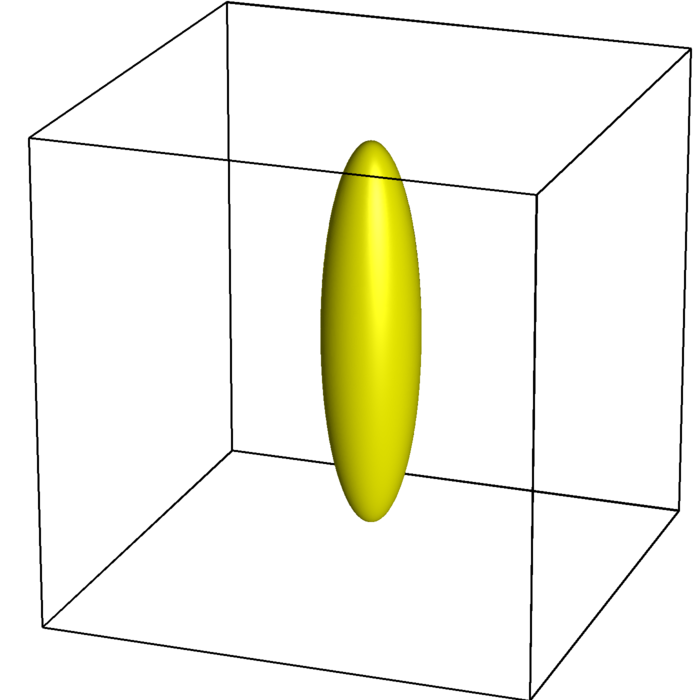
\includegraphics[width=0.3\textwidth]{images/tensor/prolate.png}
\label{fig_tensor_shapes_prolate}}
\hfill
\subfloat[Oblate ($\lambda_1 \approx \lambda_2 > \lambda_3$)]%
{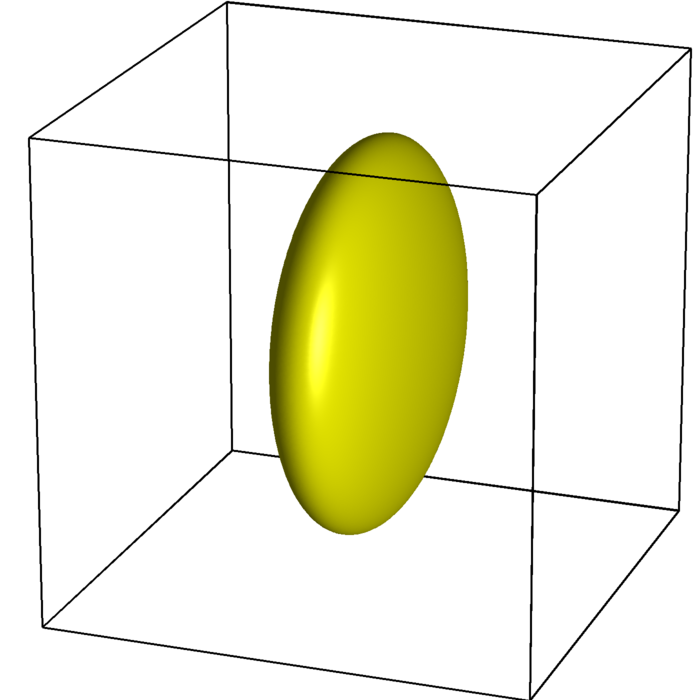
\includegraphics[width=0.3\textwidth]{images/tensor/oblate.png}
\label{fig_tensor_shapes_oblate}}
\hfill
\subfloat[Isotropic ($\lambda_1 \approx \lambda_2 \approx \lambda_3$)]%
{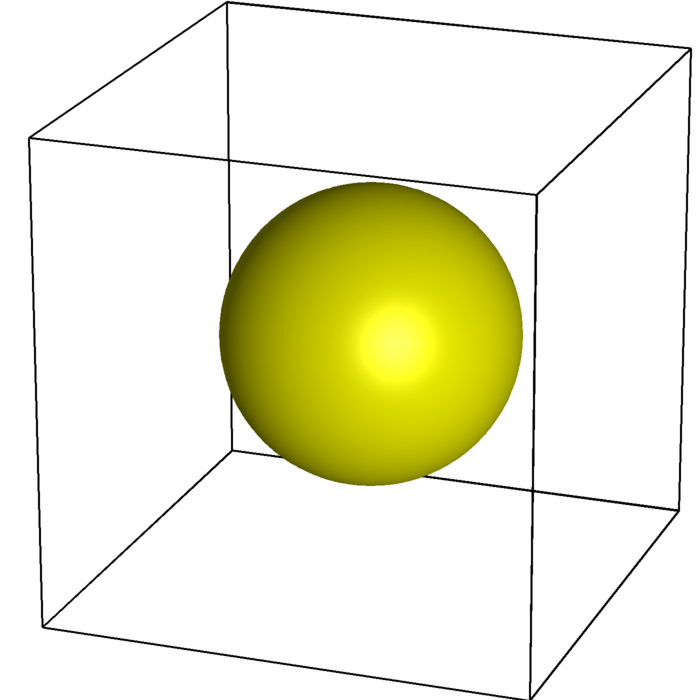
\includegraphics[width=0.3\textwidth]{images/tensor/isotropic.png}
\label{fig_tensor_shapes_isotropic}}
\caption[Shapes of the diffusion tensor governed by the relative eigenvalue amplitudes]%
{Shapes of the diffusion tensor governed by the relative eigenvalue amplitudes $\lambda_{1-3}$. When molecular diffusion is considerably larger along one particular direction, the tensor is {\em prolate} (a). If diffusion is largest on a particular plane, the tensor is {\em oblate} (b). If diffusion is equivalent in all directions, the tensor is {\em isotropic} (c).}
\label{fig_tensor_shapes}
\end{figure}%
%

The `\verb+\caption[]{}+' command within the figure environment can take two parameters, in square and curly brackets respectively. The contents of the curly brackets contents appear as the actual figure caption, while the contents of the square brackets appear in the list of figures near the start of the document. Although the latter is technically optional, I would highly recommend using this capability; make your figure captions as descriptive as possible, but make the corresponding entry in the list of figures a one-liner.

Note that it's possible to add labels to sub-figures and reference these directly, such as Figure~\ref{fig_tensor_shapes_isotropic}.

The appropriate placement of figures relative to the text can be a point of contention. In the master document (\verb+thesis.tex+), the document has been set up to prefer placement of figures at the top of the page; or where this cannot be reasonably achieved, to place one or more figures onto a page without text. To me, this is much more visually appealing than having figures appear at different vertical positions within different pages, and makes it easier for the reader to identify what text is figure legend and what is manuscript. For the examples here, I have given explicit instructions to the compiler regarding where to place these figures; on its own page (\verb+[p]+) for Figure~\ref{fig_epi_blipped}, and top of page (\verb+[t]+) for Figure~\ref{fig_tensor_shapes}.

Ideally a figure should be close to the text that references it; but again, this can't always be achieved. My approach was to place the figure code directly below the first text that references it (even if this is in the middle of a paragraph). That way, \LaTeX~will try to place the figure at the top of the page in which it is first described in the text; if this can't be done, it will place it at the top of the next page (or on a page consisting entirely of figures, if \LaTeX~deems it appropriate).

Although it's possible to have figures in \LaTeX~that don't take up the entire width of the page (e.g. by having the figure on one side of the page and the text wrapping around it, or by having the caption alongside the figure instead of below it), in my experience these are more trouble than they're worth. So I've left the necessary header files and commands out of the template. If you want to go down this road, you're on your own.

If you're generating diagram figures from scratch, I recommend the InkScape program. In addition to having all the functionalities you will need (including {\em very} handy object alignment tools), you can save the resulting figure in \verb+.pdf+ format, which will keep the file size down and won't introduce pixelation when you print (as can happen if you output to an image format). Figure~\ref{fig_epi_blipped} was produced using InkScape; even though it's a full-page figure, it's only 50KB, and doesn't pixelate no matter how much you zoom in.
%
%
\section{Table formatting}

Although tables look nice in \LaTeX, they can be awkward to construct. It's even more complicated when you want to have cells spanning multiple rows or columns. Therefore, I'm just going to provide a working example (Table~\ref{tab_sift_1}), and you can modify it as necessary.
%
\begin{table}
\centering
\begin{tabular}{c|r|r|r|r|} % Presence of vertical lines, and horizontal text alignment in each column
\cline{2-5} % Horizontal line across a subset of columns
\multirow{2}{*}{ } & \multicolumn{2}{c|}{SD\_STREAM} & \multicolumn{2}{c|}{iFOD2} \\ 
\cline{2-5}
 & White matter & GMWMI & White matter & GMWMI \\
\hline
\multicolumn{1}{|c|}{9,000,000}   &  0:08:32  &  0:06:04  &  0:14:21  &  0:08:11  \\
\multicolumn{1}{|c|}{5,000,000}   &  0:30:13  &  0:31:35  &  0:25:01  &  0:26:08  \\
\multicolumn{1}{|c|}{2,000,000}   &  1:47:24  &  2:13:34  &  0:57:14  &  1:34:02  \\
\multicolumn{1}{|c|}{Convergence} &  7:07:11  &  9:46:27  &  3:12:13  &  4:59:59  \\
\multicolumn{1}{|c|}{(remaining)} & (372,134) & (409,016) & (364,010) & (675,843) \\
\hline
\end{tabular}
\caption[Execution times for applying the SIFT algorithm]%
{Execution times for applying the SIFT algorithm to the four \invivo tractograms used in this manuscript, processed using a Core i7 machine. Tractograms differed in both the streamlines algorithm used (`SD\_STREAM' = deterministic streamlines, `iFOD2' = probabilistic streamlines), and the way in which streamlines were seeded; either throughout the white matter segmented image (`White matter') or at the \gm-\wm interface (`GMWMI'). Bracketed numbers indicate the number of streamlines remaining, after tractograms were filtered to convergence.}
\label{tab_sift_1}
\end{table}%
%
%
\section{Mathematics}

\LaTeX~excels at displaying mathematics. There's plenty of documentation on the web for how to construct and format equations. If you need to use more exotic math symbols, the Detexify\textsuperscript{2} tool may come in handy for finding the appropriate commands (\verb+http://detexify.kirelabs.org/classify.html+). TexMaker also provides common symbols in the sidebar for you to select from.

A pair of dollar-sign symbols (\verb+$...$+) defines an in-line maths environment, i.e. the equation appears within the paragraph. Only use it for very simple equations or math symbols. The `\verb+\nicefrac{}{}+' command comes in handy here, displaying fractions like $\nicefrac{1}{2}$ using a slanted line instead of a horizontal one.

A couple of example equations are provided so you can get a feel for how they look; both in the \verb+.tex+ file and in the resulting \verb+.pdf+ document. Some tricks to take note of:

\begin{itemize}
\item The caret (`\verb+^+') and underscore (`\verb+_+') symbols define superscript and subscript contents respectively; you'll probably use these often. If you don't encase the contents in curly brackets (`\verb+{}+'), only the first character following the symbol will be subscript / superscript.
\item The `\verb+\;+' command is handy for adding space between symbols in equations. There's a wide range of commands available for different spacings (even for reducing space!), but this one alone suited my needs.
\item Using \verb+align+ instead of \verb+equation+ allows you to align the horizontal position of particular symbols in multi-line equations (use the ampersand `\&' symbol to indicate the items to be aligned). Most typically these are used to align the `=' symbol for derivations, such as in Equation~\ref{eq_epi_relax_image}.
\item For multi-line equations, the `\verb+\\+' symbol indicates a new line. I recommend using \verb+\nonumber+ for all lines except the last one; this results in creation of a single reference number for the entire equation, rather than one for each individual line.
\end{itemize}

\begin{equation}
S(\mathbf{k}) = \int_V \rho(\mathbf{x}, t) e^{-i \mathbf{k} \cdot \mathbf{x}} \; d^3 \mathbf{x}
\label{eq_kspace_final}
\end{equation}

\begin{align}
s^{\text{relax}} (x_a)
&= \mathcal{F}^{-1} \lbrace S^{\text{relax}} (x_a) \rbrace \nonumber \\
&= \mathcal{F}^{-1} \lbrace S(x_a,k_{PE}) \rbrace \otimes \mathcal{F}^{-1} \lbrace e^\frac{-\epsilon_{PE} k_{PE}}{T_2^{*}(x_a)} \rbrace \nonumber \\
&= s(x_a) \otimes \frac{1}{N} \sum \limits_{k_{PE}=0}^{N-1} e^\frac{-\epsilon_{PE} k_{PE}}{T_2^{*}(x_a)} e^{\frac{2 \pi i}{N} k_{PE} x_a} \nonumber \\
&= s(x_a) \otimes \frac{1}{N} \sum \limits_{k_{PE}=0}^{N-1} e^{\frac{2 \pi i}{N} k_{PE} x_a - \Gamma \pi k_{PE}} \text{, where } \Gamma = \frac{\epsilon_{PE}}{\pi T_2^{*}} \nonumber \\
&= s(x_a) \otimes \frac{1}{\pi} \frac{0.5\Gamma}{(x-x_a)^2 + (0.5\Gamma)^2} \nonumber \\
&= s(x_a) \otimes \mathcal{L}(\Gamma)
\label{eq_epi_relax_image}
\end{align}
%
%
\section{Other tips}

This section's just an odd mish-mash of random tips and tricks that I learned along the way.

\begin{itemize}

\item The files \verb+abbrevs.tex+ and \verb+commands.tex+ provide \LaTeX~abbreviations and commands respectively. Use the `\verb+\newabbrev[]{}+' command to define common acronyms, use the command you have defined in place of that acronym, and \LaTeX~will define the acronym fully at its first appearance in the document only. Feel free to add anything to these files that you think may be useful for you.

\item The way the document is constructed from the constituent parts within the file \verb+thesis.tex+ is particularly handy for getting feedback on thesis chapters from supervisors. In \verb+thesis.tex+, you can comment out the precursor inclusions (title page, table of contents etc.), as well as the `\verb+\include{}+' commands of all chapters except the one of interest, and re-compile the document; this way, only the chapter of interest is printed to the PDF output file.

\item Unfortunately, if you have an error in one of your files and attempt to build the document, the errors that \LaTeX~gives you can be extremely cryptic. Your best option is to return the document to a state in which it does compile, and make incremental changes toward what you are trying to achieve, compiling as you go.

\item The University of Melbourne recommends a word count of around 80,000, with explicit permission required if it exceeds 100,000. You can use the program \verb+texcount+ to get the word counts of your individual chapters, exclusive of bibliography etc. (Google and download it).

\item You want to have access to the most up-to-date \verb+.tex+ files, wherever and whenever you are working. My recommendation is to use cloud storage such as Dropbox. If possible, place the \verb+.tex+ files, the \verb+.bib+ file and the \verb+images/+ directory in a synchronised location, then provide symbolic links to these files in a separate working directory; this way, the temporary files generated by the document compiler will not be synchronised (as they would be a waste of traffic). Dropbox will also keep track of previous versions of files; and if your work computer dies an abrupt death, your most prized data will be spared.

\item \LaTeX~can be prissy when it comes to file names. My recommendation is that all images and/or image sub-directories be named using lower-case letters only, and use underscores (`\_') instead of spaces. Stick to this convention, and you shouldn't have a problem. The same argument holds for use of the \verb+\label{}+ and \verb+\cite{}+ commands; you should modify your bibliography to ensure that the Bib\TeX~keys in your database are all lowercase.

\item Paragraph formatting can get weird around floats (figures and tables). I got the most consistent results by having a commented line above and below the relevant float command, and {\em also} commenting the end of the \verb+\end{figure}+ or \verb+\end{table}+ line (see examples in \verb+ch-1.tex+).

\end{itemize}

%
% The code below adds a bibliography at the end of the chapter. It assumes that your bibliography
% has been written to a file "mybib.bib". Any reference manager software should be able to write your
% bibliography in this format. If you use a different file name for your bibliography, just change the 
% code below accordingly. 
%
\cleardoublepage
\renewcommand\bibname{References}
\bibliographystyle{ieeetr}
\bibliography{mybib}
\cleardoublepage
%+' within the file \verb+thesis.tex+. Most likely, you will begin writing the first chapter of your thesis by adding your own content into this file. To add more chapters, you will need to do the following steps:

\begin{enumerate}

\item Make a copy of file \verb+ch-1.tex+, and give it a different name.

\item The new file needs to be added to the document; this is done using a corresponding `\verb+\include{}+' command within \verb+thesis.tex+.

\item You'll need to get the bibliography citations working for the new chapter also. See Section~\ref{la_citations} for details.

\end{enumerate}
%
%
\section{Text formatting}

In the file \verb+ch-1.tex+ (where the text you are reading resides), you'll notice that there's an empty line in between each paragraph. This tells \LaTeX~that these are the separations between paragraphs, and it formats them accordingly. Always include this empty line between each paragraph.

The headings of the document follow a hierarchical structure. At the top is `chapter', followed by `section', `subsection' and `subsubsection'. \LaTeX~will automatically format and number these appropriately.

\subsection{A subsection heading looks like this}

\subsubsection{And this is what the subsubsection heading looks like}

There's a few other little tips and tricks with text formatting. I'll list these using the `\verb+itemize+' environment, which displays text in bullet-point form.

\begin{itemize}

\item By default, \LaTeX~justifies the text so that it appears flush on both the left and right sides. To achieve this, it will frequently hyphenate words; however sometimes the hyphenation is not quite right. The template loads default hyphenation for the English dictionary, but it struggles with scientific terms. You can give it suggestions for hyphenation locations using the `\verb+\-+' command, e.g. \verb+hyphen\-ation+. Note that this won't force hyphenation at that point; it only provides a suggestion for the document compiler.

\item Conversely, there may be times when you want two words to appear on the same line, rather than being split between lines. This is achieved using the tilde (`$\sim$') symbol. Personally I use this whenever I reference or cite something; I use the tilde as the space between the prefix (e.g. `Section', `Figure') and the referencing command (see Section~\ref{la_referencing}), which ensures that the resulting text appears on the same line; you can see examples of this throughout the file \verb+ch-1.tex+.

\item {\bf This text is in bold font using the \verb+\bf+ command.} {\em This text is in italic (emphasis) font using the \verb+\em+ command.} \underline{This text is underlined using the} \verb+\underline+ \underline{command.}

\verb+This text is in fixed-width font using the \verb command.+

\item When placing text in `inverted commas', the start and end apostrophes are actually different characters (the opening apostrophe is to the left of the 1 key on the keyboard). The same holds for ``double inverted commas''.

\item Dashes can be of different lengths, and are generally used as follows: use single-dash for hyphenation between words; use a double dash for a numerical range e.g. 1--3; use a triple dash to separate blocks of text --- like this.

\item The percentage character (`\%') indicates a comment. Everything following that character on that particular line will be ignored by the document compiler. This is handy for making notes to yourself within the documents, or removing content without actually deleting it. It can also be used in the file \verb+thesis.tex+ to comment out those parts of the document that you don't want to be printed.

\end{itemize}

An alternative to `\verb+itemize+' is `\verb+enumerate+', which numbers items instead of just using dot points (this was used previously in the ``\nameref{la_structure}'' section). Whenever you use either of these, make sure to have the appropriate `\verb+\end{}+' command afterwards; if you don't, the document compiler will spit out an error.
%
%
\section{Internal referencing}
\label{la_referencing}

Throughout the thesis you'll need to reference sections, figures, tables etc.. This is achieved using the `\verb+\label{}+' and `\verb+\ref{}+' commands. Place a \verb+\label{}+ within the relevant content, and the corresponding \verb+\ref{}+ command will print the appropriate reference (i.e. section / figure / table number). For instance, this is Section~\ref{la_referencing}. If you change the order or placement of these labels or references, just re-compile the document and \LaTeX~will do all the re-numbering for you. Try to keep the label names meaningful; e.g. I like to use a `\verb+ch_+' prefix for chapter labels, `\verb+la_+' for general labels, `\verb+fig_+' for figures, `\verb+eq_+' for equations.
%
%
\section{Bibliography citations}
\label{la_citations}

Citations are inserted using the `\verb+\cite{}+' command. You can provide multiple citations within the same command by separating them with commas. Make sure you get the Bib\TeX~key correct, otherwise you'll get an undefined reference like this~\cite{rumpelstiltskin2013}. You can change how the citations appear (both in the manuscript and the bibliography itself) by choosing the bibliography {\em style}; this is done using the `\verb+\bibliographystyle{}+' command (see bottom of file \verb+ch-1.tex+).

The bibliography included in this template is file \verb+mybib.bib+, but only contains a single reference. Any reference management software should be capable of outputting your bibliography in \verb+.bib+ format. If you want to save your bibliography to a file with a more interesting name, you will need to modify the `\verb+bibliography{}+' command at the bottom of each chapter file accordingly.

The thesis template is configured to provide a bibliography at the end of each chapter, rather than a single massive bibliography at the end of the document. Unfortunately this does slightly complicate the compilation of the document; specifically, the \verb+bibtex+ command needs to be executed for each individual chapter.

You have three options:
%
\begin{enumerate}
\item If you use the provided \verb+build+ script, add a call to the \verb+bibtex+ command for each chapter within this script. When executed, the script will then update the per-chapter bibliographies according to any changes made.
\item The manual method is to open each individual \verb+.tex+ file in TexMaker and run Bib\TeX~manually for each (the ``Quick Build'' button is actually a drop-down menu; select Bib\TeX~from this menu, open the appropriate \verb+.tex+ file, and press the arrow button to the left of the drop-down menu). You will need to compile the document, run \verb+bibtex+ on each chapter, then re-compile again for all the citations to appear properly.
\item It may be easier to use a single large bibliography while writing the thesis, and change to per-chapter bibliographies only when it's ready to print. If you want to do this, comment out the bibliography-related stuff at the end of each chapter \verb+.tex+ file, and un-comment the relevant commands at the end of \verb+thesis.tex+. If using the provided \verb+build+ script, comment out the \verb+bibtex+ calls for the individual chapter files, and un-comment the one for \verb+thesis.tex+.
\end{enumerate}
%
%
\section{Figure formatting and placement}

The easiest way to insert new figures into the thesis is to copy-and-paste the working code for another figure, and update the fields accordingly. Figure~\ref{fig_epi_blipped} is a typical figure with a single image and caption. %
%
\begin{figure}[p]
  \centering
  \includegraphics[width=\textwidth]{images/sequences/blipped_epi.pdf}
  \caption[Pulse diagram and \kspace trajectory for single-shot blipped EPI]%
  {Pulse diagram and \kspace trajectory for single-shot blipped EPI. Pre-wind gradients in the \fe and \pe axes (A) shift the \kspace position to the corner of \kspace in preparation for readout. After a single line of \kspace is read (B), a small gradient moment is applied in the \pe direction (C) to shift the position in \kspace by a single row along this axis, and the next line of \kspace is read in the opposite direction (D). Data for the entire \kspace region is sampled following a single RF excitation. The time between successive readouts is denoted the `echo spacing' $\epsilon_{PE}$.}
  \label{fig_epi_blipped}
\end{figure}%
%
It's also possible to have multiple images in a single figure; see Figure~\ref{fig_tensor_shapes} for an example.
%
\begin{figure}[t]
\centering
\subfloat[Prolate ($\lambda_1 > \lambda_2 \approx \lambda_3$)]%
{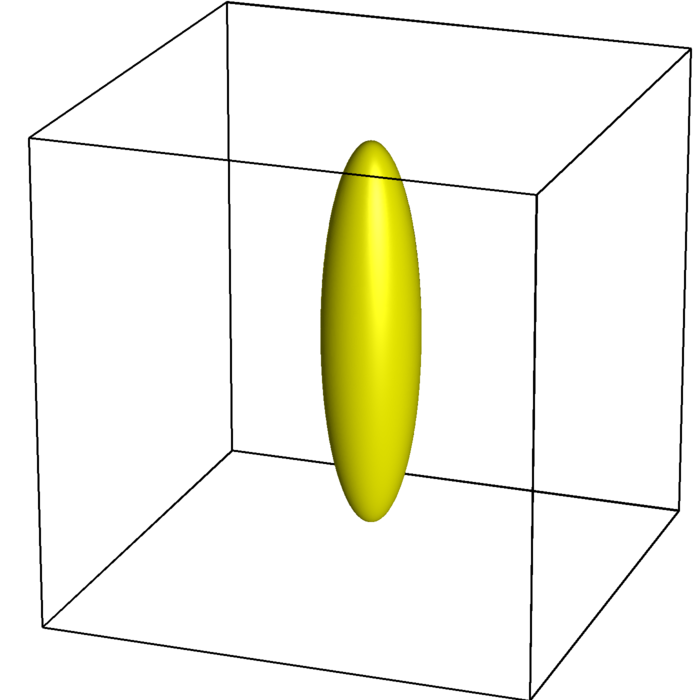
\includegraphics[width=0.3\textwidth]{images/tensor/prolate.png}
\label{fig_tensor_shapes_prolate}}
\hfill
\subfloat[Oblate ($\lambda_1 \approx \lambda_2 > \lambda_3$)]%
{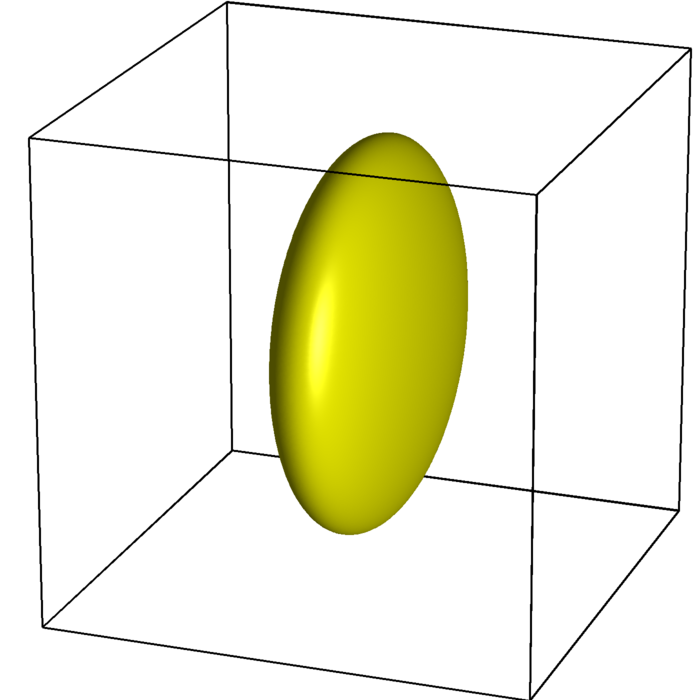
\includegraphics[width=0.3\textwidth]{images/tensor/oblate.png}
\label{fig_tensor_shapes_oblate}}
\hfill
\subfloat[Isotropic ($\lambda_1 \approx \lambda_2 \approx \lambda_3$)]%
{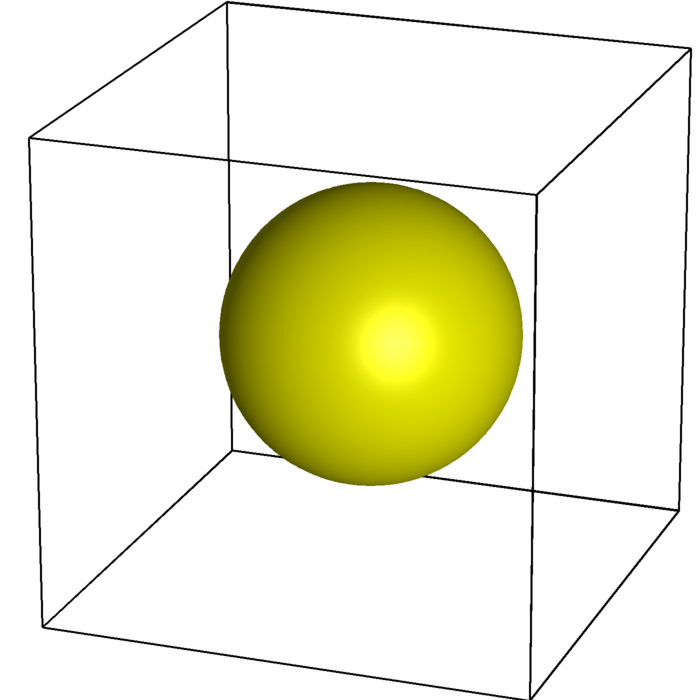
\includegraphics[width=0.3\textwidth]{images/tensor/isotropic.png}
\label{fig_tensor_shapes_isotropic}}
\caption[Shapes of the diffusion tensor governed by the relative eigenvalue amplitudes]%
{Shapes of the diffusion tensor governed by the relative eigenvalue amplitudes $\lambda_{1-3}$. When molecular diffusion is considerably larger along one particular direction, the tensor is {\em prolate} (a). If diffusion is largest on a particular plane, the tensor is {\em oblate} (b). If diffusion is equivalent in all directions, the tensor is {\em isotropic} (c).}
\label{fig_tensor_shapes}
\end{figure}%
%

The `\verb+\caption[]{}+' command within the figure environment can take two parameters, in square and curly brackets respectively. The contents of the curly brackets contents appear as the actual figure caption, while the contents of the square brackets appear in the list of figures near the start of the document. Although the latter is technically optional, I would highly recommend using this capability; make your figure captions as descriptive as possible, but make the corresponding entry in the list of figures a one-liner.

Note that it's possible to add labels to sub-figures and reference these directly, such as Figure~\ref{fig_tensor_shapes_isotropic}.

The appropriate placement of figures relative to the text can be a point of contention. In the master document (\verb+thesis.tex+), the document has been set up to prefer placement of figures at the top of the page; or where this cannot be reasonably achieved, to place one or more figures onto a page without text. To me, this is much more visually appealing than having figures appear at different vertical positions within different pages, and makes it easier for the reader to identify what text is figure legend and what is manuscript. For the examples here, I have given explicit instructions to the compiler regarding where to place these figures; on its own page (\verb+[p]+) for Figure~\ref{fig_epi_blipped}, and top of page (\verb+[t]+) for Figure~\ref{fig_tensor_shapes}.

Ideally a figure should be close to the text that references it; but again, this can't always be achieved. My approach was to place the figure code directly below the first text that references it (even if this is in the middle of a paragraph). That way, \LaTeX~will try to place the figure at the top of the page in which it is first described in the text; if this can't be done, it will place it at the top of the next page (or on a page consisting entirely of figures, if \LaTeX~deems it appropriate).

Although it's possible to have figures in \LaTeX~that don't take up the entire width of the page (e.g. by having the figure on one side of the page and the text wrapping around it, or by having the caption alongside the figure instead of below it), in my experience these are more trouble than they're worth. So I've left the necessary header files and commands out of the template. If you want to go down this road, you're on your own.

If you're generating diagram figures from scratch, I recommend the InkScape program. In addition to having all the functionalities you will need (including {\em very} handy object alignment tools), you can save the resulting figure in \verb+.pdf+ format, which will keep the file size down and won't introduce pixelation when you print (as can happen if you output to an image format). Figure~\ref{fig_epi_blipped} was produced using InkScape; even though it's a full-page figure, it's only 50KB, and doesn't pixelate no matter how much you zoom in.
%
%
\section{Table formatting}

Although tables look nice in \LaTeX, they can be awkward to construct. It's even more complicated when you want to have cells spanning multiple rows or columns. Therefore, I'm just going to provide a working example (Table~\ref{tab_sift_1}), and you can modify it as necessary.
%
\begin{table}
\centering
\begin{tabular}{c|r|r|r|r|} % Presence of vertical lines, and horizontal text alignment in each column
\cline{2-5} % Horizontal line across a subset of columns
\multirow{2}{*}{ } & \multicolumn{2}{c|}{SD\_STREAM} & \multicolumn{2}{c|}{iFOD2} \\ 
\cline{2-5}
 & White matter & GMWMI & White matter & GMWMI \\
\hline
\multicolumn{1}{|c|}{9,000,000}   &  0:08:32  &  0:06:04  &  0:14:21  &  0:08:11  \\
\multicolumn{1}{|c|}{5,000,000}   &  0:30:13  &  0:31:35  &  0:25:01  &  0:26:08  \\
\multicolumn{1}{|c|}{2,000,000}   &  1:47:24  &  2:13:34  &  0:57:14  &  1:34:02  \\
\multicolumn{1}{|c|}{Convergence} &  7:07:11  &  9:46:27  &  3:12:13  &  4:59:59  \\
\multicolumn{1}{|c|}{(remaining)} & (372,134) & (409,016) & (364,010) & (675,843) \\
\hline
\end{tabular}
\caption[Execution times for applying the SIFT algorithm]%
{Execution times for applying the SIFT algorithm to the four \invivo tractograms used in this manuscript, processed using a Core i7 machine. Tractograms differed in both the streamlines algorithm used (`SD\_STREAM' = deterministic streamlines, `iFOD2' = probabilistic streamlines), and the way in which streamlines were seeded; either throughout the white matter segmented image (`White matter') or at the \gm-\wm interface (`GMWMI'). Bracketed numbers indicate the number of streamlines remaining, after tractograms were filtered to convergence.}
\label{tab_sift_1}
\end{table}%
%
%
\section{Mathematics}

\LaTeX~excels at displaying mathematics. There's plenty of documentation on the web for how to construct and format equations. If you need to use more exotic math symbols, the Detexify\textsuperscript{2} tool may come in handy for finding the appropriate commands (\verb+http://detexify.kirelabs.org/classify.html+). TexMaker also provides common symbols in the sidebar for you to select from.

A pair of dollar-sign symbols (\verb+$...$+) defines an in-line maths environment, i.e. the equation appears within the paragraph. Only use it for very simple equations or math symbols. The `\verb+\nicefrac{}{}+' command comes in handy here, displaying fractions like $\nicefrac{1}{2}$ using a slanted line instead of a horizontal one.

A couple of example equations are provided so you can get a feel for how they look; both in the \verb+.tex+ file and in the resulting \verb+.pdf+ document. Some tricks to take note of:

\begin{itemize}
\item The caret (`\verb+^+') and underscore (`\verb+_+') symbols define superscript and subscript contents respectively; you'll probably use these often. If you don't encase the contents in curly brackets (`\verb+{}+'), only the first character following the symbol will be subscript / superscript.
\item The `\verb+\;+' command is handy for adding space between symbols in equations. There's a wide range of commands available for different spacings (even for reducing space!), but this one alone suited my needs.
\item Using \verb+align+ instead of \verb+equation+ allows you to align the horizontal position of particular symbols in multi-line equations (use the ampersand `\&' symbol to indicate the items to be aligned). Most typically these are used to align the `=' symbol for derivations, such as in Equation~\ref{eq_epi_relax_image}.
\item For multi-line equations, the `\verb+\\+' symbol indicates a new line. I recommend using \verb+\nonumber+ for all lines except the last one; this results in creation of a single reference number for the entire equation, rather than one for each individual line.
\end{itemize}

\begin{equation}
S(\mathbf{k}) = \int_V \rho(\mathbf{x}, t) e^{-i \mathbf{k} \cdot \mathbf{x}} \; d^3 \mathbf{x}
\label{eq_kspace_final}
\end{equation}

\begin{align}
s^{\text{relax}} (x_a)
&= \mathcal{F}^{-1} \lbrace S^{\text{relax}} (x_a) \rbrace \nonumber \\
&= \mathcal{F}^{-1} \lbrace S(x_a,k_{PE}) \rbrace \otimes \mathcal{F}^{-1} \lbrace e^\frac{-\epsilon_{PE} k_{PE}}{T_2^{*}(x_a)} \rbrace \nonumber \\
&= s(x_a) \otimes \frac{1}{N} \sum \limits_{k_{PE}=0}^{N-1} e^\frac{-\epsilon_{PE} k_{PE}}{T_2^{*}(x_a)} e^{\frac{2 \pi i}{N} k_{PE} x_a} \nonumber \\
&= s(x_a) \otimes \frac{1}{N} \sum \limits_{k_{PE}=0}^{N-1} e^{\frac{2 \pi i}{N} k_{PE} x_a - \Gamma \pi k_{PE}} \text{, where } \Gamma = \frac{\epsilon_{PE}}{\pi T_2^{*}} \nonumber \\
&= s(x_a) \otimes \frac{1}{\pi} \frac{0.5\Gamma}{(x-x_a)^2 + (0.5\Gamma)^2} \nonumber \\
&= s(x_a) \otimes \mathcal{L}(\Gamma)
\label{eq_epi_relax_image}
\end{align}
%
%
\section{Other tips}

This section's just an odd mish-mash of random tips and tricks that I learned along the way.

\begin{itemize}

\item The files \verb+abbrevs.tex+ and \verb+commands.tex+ provide \LaTeX~abbreviations and commands respectively. Use the `\verb+\newabbrev[]{}+' command to define common acronyms, use the command you have defined in place of that acronym, and \LaTeX~will define the acronym fully at its first appearance in the document only. Feel free to add anything to these files that you think may be useful for you.

\item The way the document is constructed from the constituent parts within the file \verb+thesis.tex+ is particularly handy for getting feedback on thesis chapters from supervisors. In \verb+thesis.tex+, you can comment out the precursor inclusions (title page, table of contents etc.), as well as the `\verb+\include{}+' commands of all chapters except the one of interest, and re-compile the document; this way, only the chapter of interest is printed to the PDF output file.

\item Unfortunately, if you have an error in one of your files and attempt to build the document, the errors that \LaTeX~gives you can be extremely cryptic. Your best option is to return the document to a state in which it does compile, and make incremental changes toward what you are trying to achieve, compiling as you go.

\item The University of Melbourne recommends a word count of around 80,000, with explicit permission required if it exceeds 100,000. You can use the program \verb+texcount+ to get the word counts of your individual chapters, exclusive of bibliography etc. (Google and download it).

\item You want to have access to the most up-to-date \verb+.tex+ files, wherever and whenever you are working. My recommendation is to use cloud storage such as Dropbox. If possible, place the \verb+.tex+ files, the \verb+.bib+ file and the \verb+images/+ directory in a synchronised location, then provide symbolic links to these files in a separate working directory; this way, the temporary files generated by the document compiler will not be synchronised (as they would be a waste of traffic). Dropbox will also keep track of previous versions of files; and if your work computer dies an abrupt death, your most prized data will be spared.

\item \LaTeX~can be prissy when it comes to file names. My recommendation is that all images and/or image sub-directories be named using lower-case letters only, and use underscores (`\_') instead of spaces. Stick to this convention, and you shouldn't have a problem. The same argument holds for use of the \verb+\label{}+ and \verb+\cite{}+ commands; you should modify your bibliography to ensure that the Bib\TeX~keys in your database are all lowercase.

\item Paragraph formatting can get weird around floats (figures and tables). I got the most consistent results by having a commented line above and below the relevant float command, and {\em also} commenting the end of the \verb+\end{figure}+ or \verb+\end{table}+ line (see examples in \verb+ch-1.tex+).

\end{itemize}

%
% The code below adds a bibliography at the end of the chapter. It assumes that your bibliography
% has been written to a file "mybib.bib". Any reference manager software should be able to write your
% bibliography in this format. If you use a different file name for your bibliography, just change the 
% code below accordingly. 
%
\cleardoublepage
\renewcommand\bibname{References}
\bibliographystyle{ieeetr}
\bibliography{mybib}
\cleardoublepage
%+' within the file \verb+thesis.tex+. Most likely, you will begin writing the first chapter of your thesis by adding your own content into this file. To add more chapters, you will need to do the following steps:

\begin{enumerate}

\item Make a copy of file \verb+ch-1.tex+, and give it a different name.

\item The new file needs to be added to the document; this is done using a corresponding `\verb+\include{}+' command within \verb+thesis.tex+.

\item You'll need to get the bibliography citations working for the new chapter also. See Section~\ref{la_citations} for details.

\end{enumerate}
%
%
\section{Text formatting}

In the file \verb+ch-1.tex+ (where the text you are reading resides), you'll notice that there's an empty line in between each paragraph. This tells \LaTeX~that these are the separations between paragraphs, and it formats them accordingly. Always include this empty line between each paragraph.

The headings of the document follow a hierarchical structure. At the top is `chapter', followed by `section', `subsection' and `subsubsection'. \LaTeX~will automatically format and number these appropriately.

\subsection{A subsection heading looks like this}

\subsubsection{And this is what the subsubsection heading looks like}

There's a few other little tips and tricks with text formatting. I'll list these using the `\verb+itemize+' environment, which displays text in bullet-point form.

\begin{itemize}

\item By default, \LaTeX~justifies the text so that it appears flush on both the left and right sides. To achieve this, it will frequently hyphenate words; however sometimes the hyphenation is not quite right. The template loads default hyphenation for the English dictionary, but it struggles with scientific terms. You can give it suggestions for hyphenation locations using the `\verb+\-+' command, e.g. \verb+hyphen\-ation+. Note that this won't force hyphenation at that point; it only provides a suggestion for the document compiler.

\item Conversely, there may be times when you want two words to appear on the same line, rather than being split between lines. This is achieved using the tilde (`$\sim$') symbol. Personally I use this whenever I reference or cite something; I use the tilde as the space between the prefix (e.g. `Section', `Figure') and the referencing command (see Section~\ref{la_referencing}), which ensures that the resulting text appears on the same line; you can see examples of this throughout the file \verb+ch-1.tex+.

\item {\bf This text is in bold font using the \verb+\bf+ command.} {\em This text is in italic (emphasis) font using the \verb+\em+ command.} \underline{This text is underlined using the} \verb+\underline+ \underline{command.}

\verb+This text is in fixed-width font using the \verb command.+

\item When placing text in `inverted commas', the start and end apostrophes are actually different characters (the opening apostrophe is to the left of the 1 key on the keyboard). The same holds for ``double inverted commas''.

\item Dashes can be of different lengths, and are generally used as follows: use single-dash for hyphenation between words; use a double dash for a numerical range e.g. 1--3; use a triple dash to separate blocks of text --- like this.

\item The percentage character (`\%') indicates a comment. Everything following that character on that particular line will be ignored by the document compiler. This is handy for making notes to yourself within the documents, or removing content without actually deleting it. It can also be used in the file \verb+thesis.tex+ to comment out those parts of the document that you don't want to be printed.

\end{itemize}

An alternative to `\verb+itemize+' is `\verb+enumerate+', which numbers items instead of just using dot points (this was used previously in the ``\nameref{la_structure}'' section). Whenever you use either of these, make sure to have the appropriate `\verb+\end{}+' command afterwards; if you don't, the document compiler will spit out an error.
%
%
\section{Internal referencing}
\label{la_referencing}

Throughout the thesis you'll need to reference sections, figures, tables etc.. This is achieved using the `\verb+\label{}+' and `\verb+\ref{}+' commands. Place a \verb+\label{}+ within the relevant content, and the corresponding \verb+\ref{}+ command will print the appropriate reference (i.e. section / figure / table number). For instance, this is Section~\ref{la_referencing}. If you change the order or placement of these labels or references, just re-compile the document and \LaTeX~will do all the re-numbering for you. Try to keep the label names meaningful; e.g. I like to use a `\verb+ch_+' prefix for chapter labels, `\verb+la_+' for general labels, `\verb+fig_+' for figures, `\verb+eq_+' for equations.
%
%
\section{Bibliography citations}
\label{la_citations}

Citations are inserted using the `\verb+\cite{}+' command. You can provide multiple citations within the same command by separating them with commas. Make sure you get the Bib\TeX~key correct, otherwise you'll get an undefined reference like this~\cite{rumpelstiltskin2013}. You can change how the citations appear (both in the manuscript and the bibliography itself) by choosing the bibliography {\em style}; this is done using the `\verb+\bibliographystyle{}+' command (see bottom of file \verb+ch-1.tex+).

The bibliography included in this template is file \verb+mybib.bib+, but only contains a single reference. Any reference management software should be capable of outputting your bibliography in \verb+.bib+ format. If you want to save your bibliography to a file with a more interesting name, you will need to modify the `\verb+bibliography{}+' command at the bottom of each chapter file accordingly.

The thesis template is configured to provide a bibliography at the end of each chapter, rather than a single massive bibliography at the end of the document. Unfortunately this does slightly complicate the compilation of the document; specifically, the \verb+bibtex+ command needs to be executed for each individual chapter.

You have three options:
%
\begin{enumerate}
\item If you use the provided \verb+build+ script, add a call to the \verb+bibtex+ command for each chapter within this script. When executed, the script will then update the per-chapter bibliographies according to any changes made.
\item The manual method is to open each individual \verb+.tex+ file in TexMaker and run Bib\TeX~manually for each (the ``Quick Build'' button is actually a drop-down menu; select Bib\TeX~from this menu, open the appropriate \verb+.tex+ file, and press the arrow button to the left of the drop-down menu). You will need to compile the document, run \verb+bibtex+ on each chapter, then re-compile again for all the citations to appear properly.
\item It may be easier to use a single large bibliography while writing the thesis, and change to per-chapter bibliographies only when it's ready to print. If you want to do this, comment out the bibliography-related stuff at the end of each chapter \verb+.tex+ file, and un-comment the relevant commands at the end of \verb+thesis.tex+. If using the provided \verb+build+ script, comment out the \verb+bibtex+ calls for the individual chapter files, and un-comment the one for \verb+thesis.tex+.
\end{enumerate}
%
%
\section{Figure formatting and placement}

The easiest way to insert new figures into the thesis is to copy-and-paste the working code for another figure, and update the fields accordingly. Figure~\ref{fig_epi_blipped} is a typical figure with a single image and caption. %
%
\begin{figure}[p]
  \centering
  \includegraphics[width=\textwidth]{images/sequences/blipped_epi.pdf}
  \caption[Pulse diagram and \kspace trajectory for single-shot blipped EPI]%
  {Pulse diagram and \kspace trajectory for single-shot blipped EPI. Pre-wind gradients in the \fe and \pe axes (A) shift the \kspace position to the corner of \kspace in preparation for readout. After a single line of \kspace is read (B), a small gradient moment is applied in the \pe direction (C) to shift the position in \kspace by a single row along this axis, and the next line of \kspace is read in the opposite direction (D). Data for the entire \kspace region is sampled following a single RF excitation. The time between successive readouts is denoted the `echo spacing' $\epsilon_{PE}$.}
  \label{fig_epi_blipped}
\end{figure}%
%
It's also possible to have multiple images in a single figure; see Figure~\ref{fig_tensor_shapes} for an example.
%
\begin{figure}[t]
\centering
\subfloat[Prolate ($\lambda_1 > \lambda_2 \approx \lambda_3$)]%
{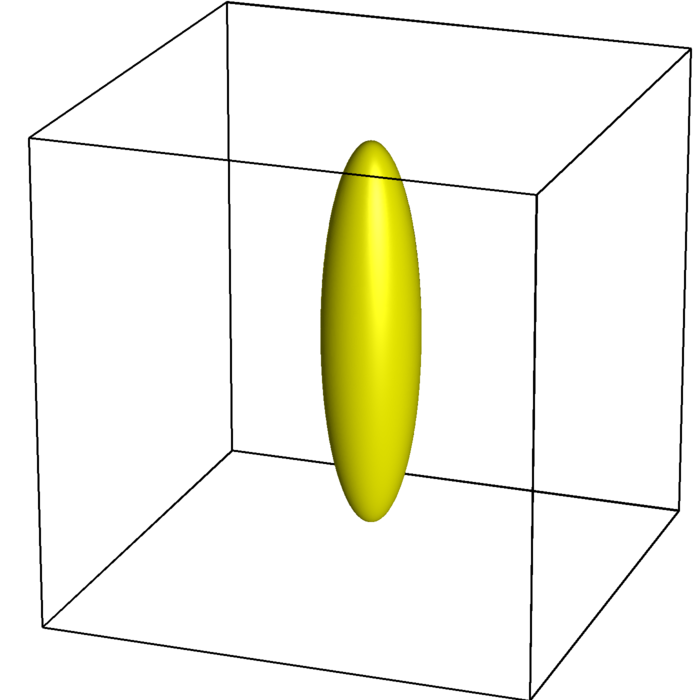
\includegraphics[width=0.3\textwidth]{images/tensor/prolate.png}
\label{fig_tensor_shapes_prolate}}
\hfill
\subfloat[Oblate ($\lambda_1 \approx \lambda_2 > \lambda_3$)]%
{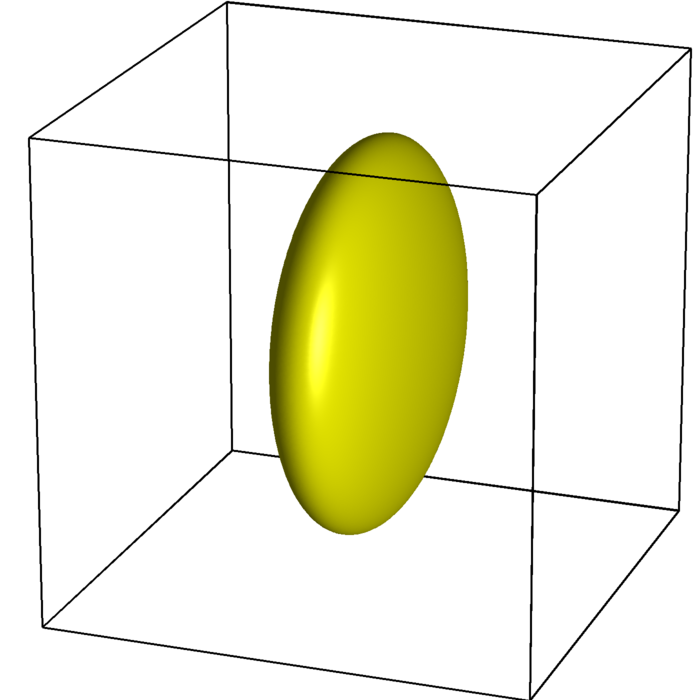
\includegraphics[width=0.3\textwidth]{images/tensor/oblate.png}
\label{fig_tensor_shapes_oblate}}
\hfill
\subfloat[Isotropic ($\lambda_1 \approx \lambda_2 \approx \lambda_3$)]%
{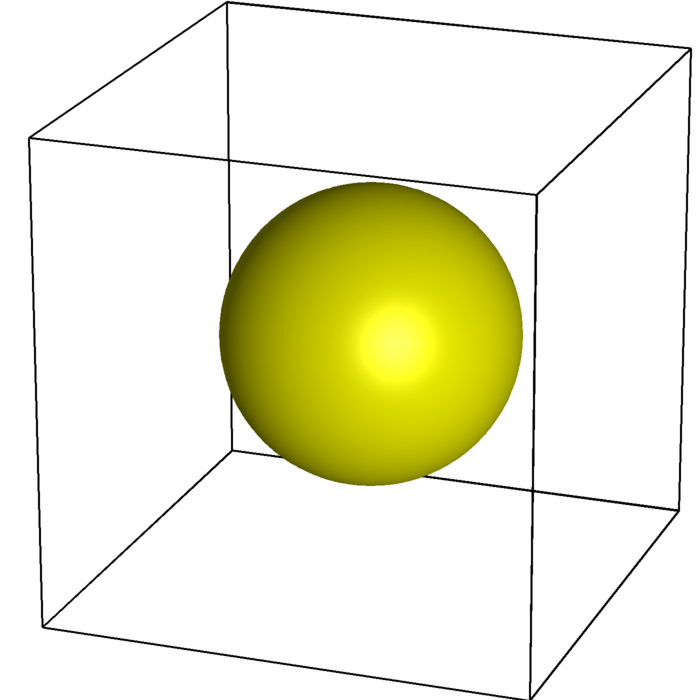
\includegraphics[width=0.3\textwidth]{images/tensor/isotropic.png}
\label{fig_tensor_shapes_isotropic}}
\caption[Shapes of the diffusion tensor governed by the relative eigenvalue amplitudes]%
{Shapes of the diffusion tensor governed by the relative eigenvalue amplitudes $\lambda_{1-3}$. When molecular diffusion is considerably larger along one particular direction, the tensor is {\em prolate} (a). If diffusion is largest on a particular plane, the tensor is {\em oblate} (b). If diffusion is equivalent in all directions, the tensor is {\em isotropic} (c).}
\label{fig_tensor_shapes}
\end{figure}%
%

The `\verb+\caption[]{}+' command within the figure environment can take two parameters, in square and curly brackets respectively. The contents of the curly brackets contents appear as the actual figure caption, while the contents of the square brackets appear in the list of figures near the start of the document. Although the latter is technically optional, I would highly recommend using this capability; make your figure captions as descriptive as possible, but make the corresponding entry in the list of figures a one-liner.

Note that it's possible to add labels to sub-figures and reference these directly, such as Figure~\ref{fig_tensor_shapes_isotropic}.

The appropriate placement of figures relative to the text can be a point of contention. In the master document (\verb+thesis.tex+), the document has been set up to prefer placement of figures at the top of the page; or where this cannot be reasonably achieved, to place one or more figures onto a page without text. To me, this is much more visually appealing than having figures appear at different vertical positions within different pages, and makes it easier for the reader to identify what text is figure legend and what is manuscript. For the examples here, I have given explicit instructions to the compiler regarding where to place these figures; on its own page (\verb+[p]+) for Figure~\ref{fig_epi_blipped}, and top of page (\verb+[t]+) for Figure~\ref{fig_tensor_shapes}.

Ideally a figure should be close to the text that references it; but again, this can't always be achieved. My approach was to place the figure code directly below the first text that references it (even if this is in the middle of a paragraph). That way, \LaTeX~will try to place the figure at the top of the page in which it is first described in the text; if this can't be done, it will place it at the top of the next page (or on a page consisting entirely of figures, if \LaTeX~deems it appropriate).

Although it's possible to have figures in \LaTeX~that don't take up the entire width of the page (e.g. by having the figure on one side of the page and the text wrapping around it, or by having the caption alongside the figure instead of below it), in my experience these are more trouble than they're worth. So I've left the necessary header files and commands out of the template. If you want to go down this road, you're on your own.

If you're generating diagram figures from scratch, I recommend the InkScape program. In addition to having all the functionalities you will need (including {\em very} handy object alignment tools), you can save the resulting figure in \verb+.pdf+ format, which will keep the file size down and won't introduce pixelation when you print (as can happen if you output to an image format). Figure~\ref{fig_epi_blipped} was produced using InkScape; even though it's a full-page figure, it's only 50KB, and doesn't pixelate no matter how much you zoom in.
%
%
\section{Table formatting}

Although tables look nice in \LaTeX, they can be awkward to construct. It's even more complicated when you want to have cells spanning multiple rows or columns. Therefore, I'm just going to provide a working example (Table~\ref{tab_sift_1}), and you can modify it as necessary.
%
\begin{table}
\centering
\begin{tabular}{c|r|r|r|r|} % Presence of vertical lines, and horizontal text alignment in each column
\cline{2-5} % Horizontal line across a subset of columns
\multirow{2}{*}{ } & \multicolumn{2}{c|}{SD\_STREAM} & \multicolumn{2}{c|}{iFOD2} \\ 
\cline{2-5}
 & White matter & GMWMI & White matter & GMWMI \\
\hline
\multicolumn{1}{|c|}{9,000,000}   &  0:08:32  &  0:06:04  &  0:14:21  &  0:08:11  \\
\multicolumn{1}{|c|}{5,000,000}   &  0:30:13  &  0:31:35  &  0:25:01  &  0:26:08  \\
\multicolumn{1}{|c|}{2,000,000}   &  1:47:24  &  2:13:34  &  0:57:14  &  1:34:02  \\
\multicolumn{1}{|c|}{Convergence} &  7:07:11  &  9:46:27  &  3:12:13  &  4:59:59  \\
\multicolumn{1}{|c|}{(remaining)} & (372,134) & (409,016) & (364,010) & (675,843) \\
\hline
\end{tabular}
\caption[Execution times for applying the SIFT algorithm]%
{Execution times for applying the SIFT algorithm to the four \invivo tractograms used in this manuscript, processed using a Core i7 machine. Tractograms differed in both the streamlines algorithm used (`SD\_STREAM' = deterministic streamlines, `iFOD2' = probabilistic streamlines), and the way in which streamlines were seeded; either throughout the white matter segmented image (`White matter') or at the \gm-\wm interface (`GMWMI'). Bracketed numbers indicate the number of streamlines remaining, after tractograms were filtered to convergence.}
\label{tab_sift_1}
\end{table}%
%
%
\section{Mathematics}

\LaTeX~excels at displaying mathematics. There's plenty of documentation on the web for how to construct and format equations. If you need to use more exotic math symbols, the Detexify\textsuperscript{2} tool may come in handy for finding the appropriate commands (\verb+http://detexify.kirelabs.org/classify.html+). TexMaker also provides common symbols in the sidebar for you to select from.

A pair of dollar-sign symbols (\verb+$...$+) defines an in-line maths environment, i.e. the equation appears within the paragraph. Only use it for very simple equations or math symbols. The `\verb+\nicefrac{}{}+' command comes in handy here, displaying fractions like $\nicefrac{1}{2}$ using a slanted line instead of a horizontal one.

A couple of example equations are provided so you can get a feel for how they look; both in the \verb+.tex+ file and in the resulting \verb+.pdf+ document. Some tricks to take note of:

\begin{itemize}
\item The caret (`\verb+^+') and underscore (`\verb+_+') symbols define superscript and subscript contents respectively; you'll probably use these often. If you don't encase the contents in curly brackets (`\verb+{}+'), only the first character following the symbol will be subscript / superscript.
\item The `\verb+\;+' command is handy for adding space between symbols in equations. There's a wide range of commands available for different spacings (even for reducing space!), but this one alone suited my needs.
\item Using \verb+align+ instead of \verb+equation+ allows you to align the horizontal position of particular symbols in multi-line equations (use the ampersand `\&' symbol to indicate the items to be aligned). Most typically these are used to align the `=' symbol for derivations, such as in Equation~\ref{eq_epi_relax_image}.
\item For multi-line equations, the `\verb+\\+' symbol indicates a new line. I recommend using \verb+\nonumber+ for all lines except the last one; this results in creation of a single reference number for the entire equation, rather than one for each individual line.
\end{itemize}

\begin{equation}
S(\mathbf{k}) = \int_V \rho(\mathbf{x}, t) e^{-i \mathbf{k} \cdot \mathbf{x}} \; d^3 \mathbf{x}
\label{eq_kspace_final}
\end{equation}

\begin{align}
s^{\text{relax}} (x_a)
&= \mathcal{F}^{-1} \lbrace S^{\text{relax}} (x_a) \rbrace \nonumber \\
&= \mathcal{F}^{-1} \lbrace S(x_a,k_{PE}) \rbrace \otimes \mathcal{F}^{-1} \lbrace e^\frac{-\epsilon_{PE} k_{PE}}{T_2^{*}(x_a)} \rbrace \nonumber \\
&= s(x_a) \otimes \frac{1}{N} \sum \limits_{k_{PE}=0}^{N-1} e^\frac{-\epsilon_{PE} k_{PE}}{T_2^{*}(x_a)} e^{\frac{2 \pi i}{N} k_{PE} x_a} \nonumber \\
&= s(x_a) \otimes \frac{1}{N} \sum \limits_{k_{PE}=0}^{N-1} e^{\frac{2 \pi i}{N} k_{PE} x_a - \Gamma \pi k_{PE}} \text{, where } \Gamma = \frac{\epsilon_{PE}}{\pi T_2^{*}} \nonumber \\
&= s(x_a) \otimes \frac{1}{\pi} \frac{0.5\Gamma}{(x-x_a)^2 + (0.5\Gamma)^2} \nonumber \\
&= s(x_a) \otimes \mathcal{L}(\Gamma)
\label{eq_epi_relax_image}
\end{align}
%
%
\section{Other tips}

This section's just an odd mish-mash of random tips and tricks that I learned along the way.

\begin{itemize}

\item The files \verb+abbrevs.tex+ and \verb+commands.tex+ provide \LaTeX~abbreviations and commands respectively. Use the `\verb+\newabbrev[]{}+' command to define common acronyms, use the command you have defined in place of that acronym, and \LaTeX~will define the acronym fully at its first appearance in the document only. Feel free to add anything to these files that you think may be useful for you.

\item The way the document is constructed from the constituent parts within the file \verb+thesis.tex+ is particularly handy for getting feedback on thesis chapters from supervisors. In \verb+thesis.tex+, you can comment out the precursor inclusions (title page, table of contents etc.), as well as the `\verb+\include{}+' commands of all chapters except the one of interest, and re-compile the document; this way, only the chapter of interest is printed to the PDF output file.

\item Unfortunately, if you have an error in one of your files and attempt to build the document, the errors that \LaTeX~gives you can be extremely cryptic. Your best option is to return the document to a state in which it does compile, and make incremental changes toward what you are trying to achieve, compiling as you go.

\item The University of Melbourne recommends a word count of around 80,000, with explicit permission required if it exceeds 100,000. You can use the program \verb+texcount+ to get the word counts of your individual chapters, exclusive of bibliography etc. (Google and download it).

\item You want to have access to the most up-to-date \verb+.tex+ files, wherever and whenever you are working. My recommendation is to use cloud storage such as Dropbox. If possible, place the \verb+.tex+ files, the \verb+.bib+ file and the \verb+images/+ directory in a synchronised location, then provide symbolic links to these files in a separate working directory; this way, the temporary files generated by the document compiler will not be synchronised (as they would be a waste of traffic). Dropbox will also keep track of previous versions of files; and if your work computer dies an abrupt death, your most prized data will be spared.

\item \LaTeX~can be prissy when it comes to file names. My recommendation is that all images and/or image sub-directories be named using lower-case letters only, and use underscores (`\_') instead of spaces. Stick to this convention, and you shouldn't have a problem. The same argument holds for use of the \verb+\label{}+ and \verb+\cite{}+ commands; you should modify your bibliography to ensure that the Bib\TeX~keys in your database are all lowercase.

\item Paragraph formatting can get weird around floats (figures and tables). I got the most consistent results by having a commented line above and below the relevant float command, and {\em also} commenting the end of the \verb+\end{figure}+ or \verb+\end{table}+ line (see examples in \verb+ch-1.tex+).

\end{itemize}

%
% The code below adds a bibliography at the end of the chapter. It assumes that your bibliography
% has been written to a file "mybib.bib". Any reference manager software should be able to write your
% bibliography in this format. If you use a different file name for your bibliography, just change the 
% code below accordingly. 
%
\cleardoublepage
\renewcommand\bibname{References}
\bibliographystyle{ieeetr}
\bibliography{mybib}
\cleardoublepage
%+' within the file \verb+thesis.tex+. Most likely, you will begin writing the first chapter of your thesis by adding your own content into this file. To add more chapters, you will need to do the following steps:

\begin{enumerate}

\item Make a copy of file \verb+ch-1.tex+, and give it a different name.

\item The new file needs to be added to the document; this is done using a corresponding `\verb+\include{}+' command within \verb+thesis.tex+.

\item You'll need to get the bibliography citations working for the new chapter also. See Section~\ref{la_citations} for details.

\end{enumerate}
%
%
\section{Text formatting}

In the file \verb+ch-1.tex+ (where the text you are reading resides), you'll notice that there's an empty line in between each paragraph. This tells \LaTeX~that these are the separations between paragraphs, and it formats them accordingly. Always include this empty line between each paragraph.

The headings of the document follow a hierarchical structure. At the top is `chapter', followed by `section', `subsection' and `subsubsection'. \LaTeX~will automatically format and number these appropriately.

\subsection{A subsection heading looks like this}

\subsubsection{And this is what the subsubsection heading looks like}

There's a few other little tips and tricks with text formatting. I'll list these using the `\verb+itemize+' environment, which displays text in bullet-point form.

\begin{itemize}

\item By default, \LaTeX~justifies the text so that it appears flush on both the left and right sides. To achieve this, it will frequently hyphenate words; however sometimes the hyphenation is not quite right. The template loads default hyphenation for the English dictionary, but it struggles with scientific terms. You can give it suggestions for hyphenation locations using the `\verb+\-+' command, e.g. \verb+hyphen\-ation+. Note that this won't force hyphenation at that point; it only provides a suggestion for the document compiler.

\item Conversely, there may be times when you want two words to appear on the same line, rather than being split between lines. This is achieved using the tilde (`$\sim$') symbol. Personally I use this whenever I reference or cite something; I use the tilde as the space between the prefix (e.g. `Section', `Figure') and the referencing command (see Section~\ref{la_referencing}), which ensures that the resulting text appears on the same line; you can see examples of this throughout the file \verb+ch-1.tex+.

\item {\bf This text is in bold font using the \verb+\bf+ command.} {\em This text is in italic (emphasis) font using the \verb+\em+ command.} \underline{This text is underlined using the} \verb+\underline+ \underline{command.}

\verb+This text is in fixed-width font using the \verb command.+

\item When placing text in `inverted commas', the start and end apostrophes are actually different characters (the opening apostrophe is to the left of the 1 key on the keyboard). The same holds for ``double inverted commas''.

\item Dashes can be of different lengths, and are generally used as follows: use single-dash for hyphenation between words; use a double dash for a numerical range e.g. 1--3; use a triple dash to separate blocks of text --- like this.

\item The percentage character (`\%') indicates a comment. Everything following that character on that particular line will be ignored by the document compiler. This is handy for making notes to yourself within the documents, or removing content without actually deleting it. It can also be used in the file \verb+thesis.tex+ to comment out those parts of the document that you don't want to be printed.

\end{itemize}

An alternative to `\verb+itemize+' is `\verb+enumerate+', which numbers items instead of just using dot points (this was used previously in the ``\nameref{la_structure}'' section). Whenever you use either of these, make sure to have the appropriate `\verb+\end{}+' command afterwards; if you don't, the document compiler will spit out an error.
%
%
\section{Internal referencing}
\label{la_referencing}

Throughout the thesis you'll need to reference sections, figures, tables etc.. This is achieved using the `\verb+\label{}+' and `\verb+\ref{}+' commands. Place a \verb+\label{}+ within the relevant content, and the corresponding \verb+\ref{}+ command will print the appropriate reference (i.e. section / figure / table number). For instance, this is Section~\ref{la_referencing}. If you change the order or placement of these labels or references, just re-compile the document and \LaTeX~will do all the re-numbering for you. Try to keep the label names meaningful; e.g. I like to use a `\verb+ch_+' prefix for chapter labels, `\verb+la_+' for general labels, `\verb+fig_+' for figures, `\verb+eq_+' for equations.
%
%
\section{Bibliography citations}
\label{la_citations}

Citations are inserted using the `\verb+\cite{}+' command. You can provide multiple citations within the same command by separating them with commas. Make sure you get the Bib\TeX~key correct, otherwise you'll get an undefined reference like this~\cite{rumpelstiltskin2013}. You can change how the citations appear (both in the manuscript and the bibliography itself) by choosing the bibliography {\em style}; this is done using the `\verb+\bibliographystyle{}+' command (see bottom of file \verb+ch-1.tex+).

The bibliography included in this template is file \verb+mybib.bib+, but only contains a single reference. Any reference management software should be capable of outputting your bibliography in \verb+.bib+ format. If you want to save your bibliography to a file with a more interesting name, you will need to modify the `\verb+bibliography{}+' command at the bottom of each chapter file accordingly.

The thesis template is configured to provide a bibliography at the end of each chapter, rather than a single massive bibliography at the end of the document. Unfortunately this does slightly complicate the compilation of the document; specifically, the \verb+bibtex+ command needs to be executed for each individual chapter.

You have three options:
%
\begin{enumerate}
\item If you use the provided \verb+build+ script, add a call to the \verb+bibtex+ command for each chapter within this script. When executed, the script will then update the per-chapter bibliographies according to any changes made.
\item The manual method is to open each individual \verb+.tex+ file in TexMaker and run Bib\TeX~manually for each (the ``Quick Build'' button is actually a drop-down menu; select Bib\TeX~from this menu, open the appropriate \verb+.tex+ file, and press the arrow button to the left of the drop-down menu). You will need to compile the document, run \verb+bibtex+ on each chapter, then re-compile again for all the citations to appear properly.
\item It may be easier to use a single large bibliography while writing the thesis, and change to per-chapter bibliographies only when it's ready to print. If you want to do this, comment out the bibliography-related stuff at the end of each chapter \verb+.tex+ file, and un-comment the relevant commands at the end of \verb+thesis.tex+. If using the provided \verb+build+ script, comment out the \verb+bibtex+ calls for the individual chapter files, and un-comment the one for \verb+thesis.tex+.
\end{enumerate}
%
%
\section{Figure formatting and placement}

The easiest way to insert new figures into the thesis is to copy-and-paste the working code for another figure, and update the fields accordingly. Figure~\ref{fig_epi_blipped} is a typical figure with a single image and caption. %
%
\begin{figure}[p]
  \centering
  \includegraphics[width=\textwidth]{images/sequences/blipped_epi.pdf}
  \caption[Pulse diagram and \kspace trajectory for single-shot blipped EPI]%
  {Pulse diagram and \kspace trajectory for single-shot blipped EPI. Pre-wind gradients in the \fe and \pe axes (A) shift the \kspace position to the corner of \kspace in preparation for readout. After a single line of \kspace is read (B), a small gradient moment is applied in the \pe direction (C) to shift the position in \kspace by a single row along this axis, and the next line of \kspace is read in the opposite direction (D). Data for the entire \kspace region is sampled following a single RF excitation. The time between successive readouts is denoted the `echo spacing' $\epsilon_{PE}$.}
  \label{fig_epi_blipped}
\end{figure}%
%
It's also possible to have multiple images in a single figure; see Figure~\ref{fig_tensor_shapes} for an example.
%
\begin{figure}[t]
\centering
\subfloat[Prolate ($\lambda_1 > \lambda_2 \approx \lambda_3$)]%
{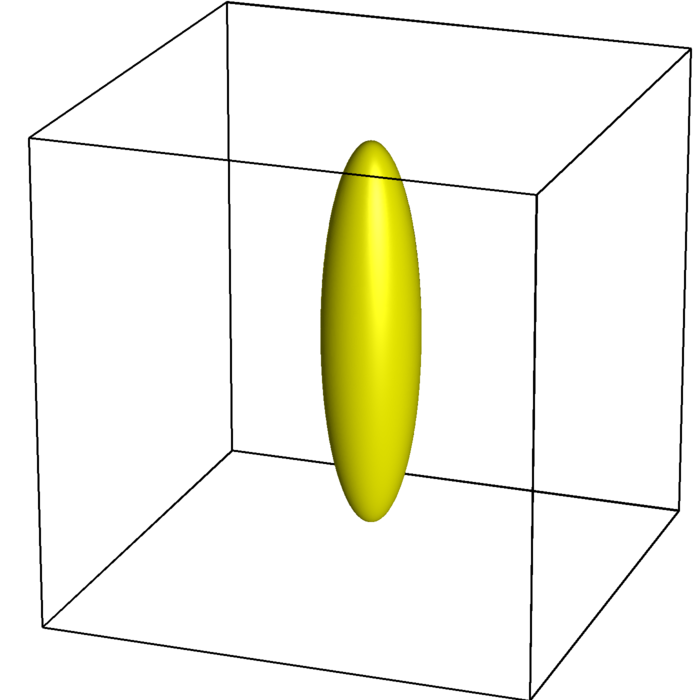
\includegraphics[width=0.3\textwidth]{images/tensor/prolate.png}
\label{fig_tensor_shapes_prolate}}
\hfill
\subfloat[Oblate ($\lambda_1 \approx \lambda_2 > \lambda_3$)]%
{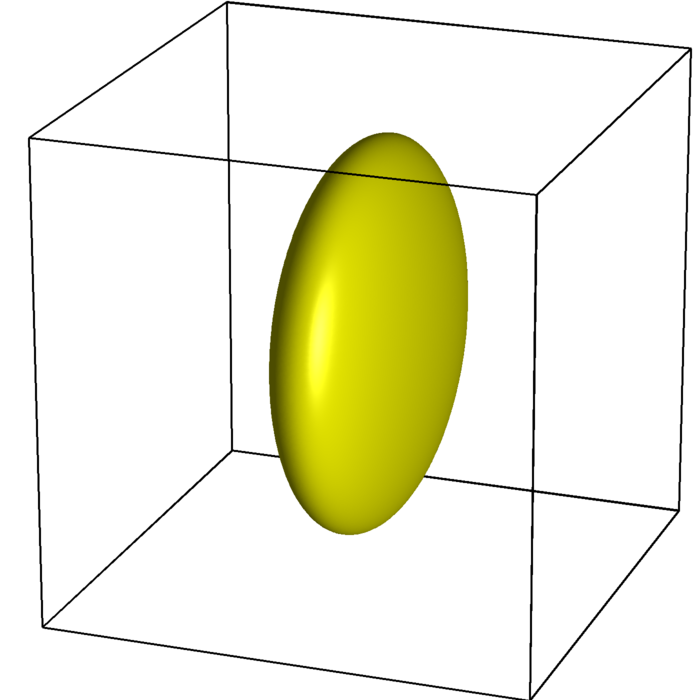
\includegraphics[width=0.3\textwidth]{images/tensor/oblate.png}
\label{fig_tensor_shapes_oblate}}
\hfill
\subfloat[Isotropic ($\lambda_1 \approx \lambda_2 \approx \lambda_3$)]%
{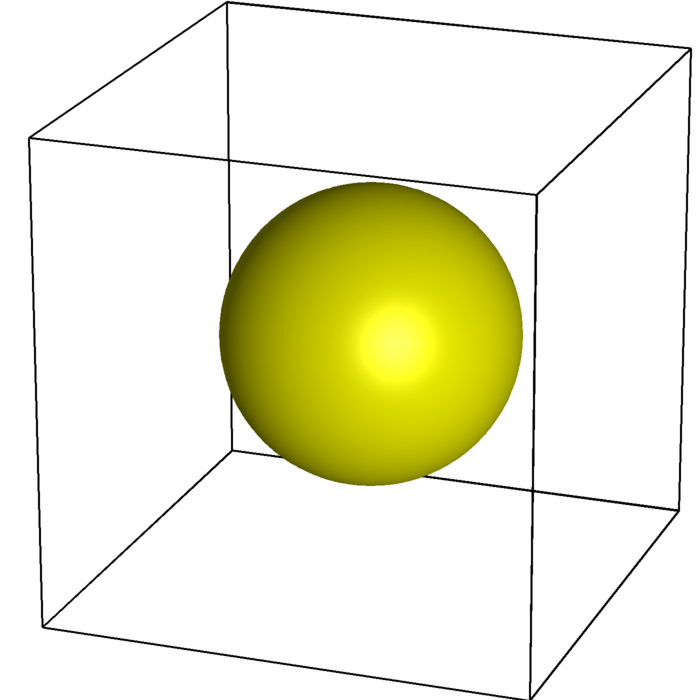
\includegraphics[width=0.3\textwidth]{images/tensor/isotropic.png}
\label{fig_tensor_shapes_isotropic}}
\caption[Shapes of the diffusion tensor governed by the relative eigenvalue amplitudes]%
{Shapes of the diffusion tensor governed by the relative eigenvalue amplitudes $\lambda_{1-3}$. When molecular diffusion is considerably larger along one particular direction, the tensor is {\em prolate} (a). If diffusion is largest on a particular plane, the tensor is {\em oblate} (b). If diffusion is equivalent in all directions, the tensor is {\em isotropic} (c).}
\label{fig_tensor_shapes}
\end{figure}%
%

The `\verb+\caption[]{}+' command within the figure environment can take two parameters, in square and curly brackets respectively. The contents of the curly brackets contents appear as the actual figure caption, while the contents of the square brackets appear in the list of figures near the start of the document. Although the latter is technically optional, I would highly recommend using this capability; make your figure captions as descriptive as possible, but make the corresponding entry in the list of figures a one-liner.

Note that it's possible to add labels to sub-figures and reference these directly, such as Figure~\ref{fig_tensor_shapes_isotropic}.

The appropriate placement of figures relative to the text can be a point of contention. In the master document (\verb+thesis.tex+), the document has been set up to prefer placement of figures at the top of the page; or where this cannot be reasonably achieved, to place one or more figures onto a page without text. To me, this is much more visually appealing than having figures appear at different vertical positions within different pages, and makes it easier for the reader to identify what text is figure legend and what is manuscript. For the examples here, I have given explicit instructions to the compiler regarding where to place these figures; on its own page (\verb+[p]+) for Figure~\ref{fig_epi_blipped}, and top of page (\verb+[t]+) for Figure~\ref{fig_tensor_shapes}.

Ideally a figure should be close to the text that references it; but again, this can't always be achieved. My approach was to place the figure code directly below the first text that references it (even if this is in the middle of a paragraph). That way, \LaTeX~will try to place the figure at the top of the page in which it is first described in the text; if this can't be done, it will place it at the top of the next page (or on a page consisting entirely of figures, if \LaTeX~deems it appropriate).

Although it's possible to have figures in \LaTeX~that don't take up the entire width of the page (e.g. by having the figure on one side of the page and the text wrapping around it, or by having the caption alongside the figure instead of below it), in my experience these are more trouble than they're worth. So I've left the necessary header files and commands out of the template. If you want to go down this road, you're on your own.

If you're generating diagram figures from scratch, I recommend the InkScape program. In addition to having all the functionalities you will need (including {\em very} handy object alignment tools), you can save the resulting figure in \verb+.pdf+ format, which will keep the file size down and won't introduce pixelation when you print (as can happen if you output to an image format). Figure~\ref{fig_epi_blipped} was produced using InkScape; even though it's a full-page figure, it's only 50KB, and doesn't pixelate no matter how much you zoom in.
%
%
\section{Table formatting}

Although tables look nice in \LaTeX, they can be awkward to construct. It's even more complicated when you want to have cells spanning multiple rows or columns. Therefore, I'm just going to provide a working example (Table~\ref{tab_sift_1}), and you can modify it as necessary.
%
\begin{table}
\centering
\begin{tabular}{c|r|r|r|r|} % Presence of vertical lines, and horizontal text alignment in each column
\cline{2-5} % Horizontal line across a subset of columns
\multirow{2}{*}{ } & \multicolumn{2}{c|}{SD\_STREAM} & \multicolumn{2}{c|}{iFOD2} \\ 
\cline{2-5}
 & White matter & GMWMI & White matter & GMWMI \\
\hline
\multicolumn{1}{|c|}{9,000,000}   &  0:08:32  &  0:06:04  &  0:14:21  &  0:08:11  \\
\multicolumn{1}{|c|}{5,000,000}   &  0:30:13  &  0:31:35  &  0:25:01  &  0:26:08  \\
\multicolumn{1}{|c|}{2,000,000}   &  1:47:24  &  2:13:34  &  0:57:14  &  1:34:02  \\
\multicolumn{1}{|c|}{Convergence} &  7:07:11  &  9:46:27  &  3:12:13  &  4:59:59  \\
\multicolumn{1}{|c|}{(remaining)} & (372,134) & (409,016) & (364,010) & (675,843) \\
\hline
\end{tabular}
\caption[Execution times for applying the SIFT algorithm]%
{Execution times for applying the SIFT algorithm to the four \invivo tractograms used in this manuscript, processed using a Core i7 machine. Tractograms differed in both the streamlines algorithm used (`SD\_STREAM' = deterministic streamlines, `iFOD2' = probabilistic streamlines), and the way in which streamlines were seeded; either throughout the white matter segmented image (`White matter') or at the \gm-\wm interface (`GMWMI'). Bracketed numbers indicate the number of streamlines remaining, after tractograms were filtered to convergence.}
\label{tab_sift_1}
\end{table}%
%
%
\section{Mathematics}

\LaTeX~excels at displaying mathematics. There's plenty of documentation on the web for how to construct and format equations. If you need to use more exotic math symbols, the Detexify\textsuperscript{2} tool may come in handy for finding the appropriate commands (\verb+http://detexify.kirelabs.org/classify.html+). TexMaker also provides common symbols in the sidebar for you to select from.

A pair of dollar-sign symbols (\verb+$...$+) defines an in-line maths environment, i.e. the equation appears within the paragraph. Only use it for very simple equations or math symbols. The `\verb+\nicefrac{}{}+' command comes in handy here, displaying fractions like $\nicefrac{1}{2}$ using a slanted line instead of a horizontal one.

A couple of example equations are provided so you can get a feel for how they look; both in the \verb+.tex+ file and in the resulting \verb+.pdf+ document. Some tricks to take note of:

\begin{itemize}
\item The caret (`\verb+^+') and underscore (`\verb+_+') symbols define superscript and subscript contents respectively; you'll probably use these often. If you don't encase the contents in curly brackets (`\verb+{}+'), only the first character following the symbol will be subscript / superscript.
\item The `\verb+\;+' command is handy for adding space between symbols in equations. There's a wide range of commands available for different spacings (even for reducing space!), but this one alone suited my needs.
\item Using \verb+align+ instead of \verb+equation+ allows you to align the horizontal position of particular symbols in multi-line equations (use the ampersand `\&' symbol to indicate the items to be aligned). Most typically these are used to align the `=' symbol for derivations, such as in Equation~\ref{eq_epi_relax_image}.
\item For multi-line equations, the `\verb+\\+' symbol indicates a new line. I recommend using \verb+\nonumber+ for all lines except the last one; this results in creation of a single reference number for the entire equation, rather than one for each individual line.
\end{itemize}

\begin{equation}
S(\mathbf{k}) = \int_V \rho(\mathbf{x}, t) e^{-i \mathbf{k} \cdot \mathbf{x}} \; d^3 \mathbf{x}
\label{eq_kspace_final}
\end{equation}

\begin{align}
s^{\text{relax}} (x_a)
&= \mathcal{F}^{-1} \lbrace S^{\text{relax}} (x_a) \rbrace \nonumber \\
&= \mathcal{F}^{-1} \lbrace S(x_a,k_{PE}) \rbrace \otimes \mathcal{F}^{-1} \lbrace e^\frac{-\epsilon_{PE} k_{PE}}{T_2^{*}(x_a)} \rbrace \nonumber \\
&= s(x_a) \otimes \frac{1}{N} \sum \limits_{k_{PE}=0}^{N-1} e^\frac{-\epsilon_{PE} k_{PE}}{T_2^{*}(x_a)} e^{\frac{2 \pi i}{N} k_{PE} x_a} \nonumber \\
&= s(x_a) \otimes \frac{1}{N} \sum \limits_{k_{PE}=0}^{N-1} e^{\frac{2 \pi i}{N} k_{PE} x_a - \Gamma \pi k_{PE}} \text{, where } \Gamma = \frac{\epsilon_{PE}}{\pi T_2^{*}} \nonumber \\
&= s(x_a) \otimes \frac{1}{\pi} \frac{0.5\Gamma}{(x-x_a)^2 + (0.5\Gamma)^2} \nonumber \\
&= s(x_a) \otimes \mathcal{L}(\Gamma)
\label{eq_epi_relax_image}
\end{align}
%
%
\section{Other tips}

This section's just an odd mish-mash of random tips and tricks that I learned along the way.

\begin{itemize}

\item The files \verb+abbrevs.tex+ and \verb+commands.tex+ provide \LaTeX~abbreviations and commands respectively. Use the `\verb+\newabbrev[]{}+' command to define common acronyms, use the command you have defined in place of that acronym, and \LaTeX~will define the acronym fully at its first appearance in the document only. Feel free to add anything to these files that you think may be useful for you.

\item The way the document is constructed from the constituent parts within the file \verb+thesis.tex+ is particularly handy for getting feedback on thesis chapters from supervisors. In \verb+thesis.tex+, you can comment out the precursor inclusions (title page, table of contents etc.), as well as the `\verb+\include{}+' commands of all chapters except the one of interest, and re-compile the document; this way, only the chapter of interest is printed to the PDF output file.

\item Unfortunately, if you have an error in one of your files and attempt to build the document, the errors that \LaTeX~gives you can be extremely cryptic. Your best option is to return the document to a state in which it does compile, and make incremental changes toward what you are trying to achieve, compiling as you go.

\item The University of Melbourne recommends a word count of around 80,000, with explicit permission required if it exceeds 100,000. You can use the program \verb+texcount+ to get the word counts of your individual chapters, exclusive of bibliography etc. (Google and download it).

\item You want to have access to the most up-to-date \verb+.tex+ files, wherever and whenever you are working. My recommendation is to use cloud storage such as Dropbox. If possible, place the \verb+.tex+ files, the \verb+.bib+ file and the \verb+images/+ directory in a synchronised location, then provide symbolic links to these files in a separate working directory; this way, the temporary files generated by the document compiler will not be synchronised (as they would be a waste of traffic). Dropbox will also keep track of previous versions of files; and if your work computer dies an abrupt death, your most prized data will be spared.

\item \LaTeX~can be prissy when it comes to file names. My recommendation is that all images and/or image sub-directories be named using lower-case letters only, and use underscores (`\_') instead of spaces. Stick to this convention, and you shouldn't have a problem. The same argument holds for use of the \verb+\label{}+ and \verb+\cite{}+ commands; you should modify your bibliography to ensure that the Bib\TeX~keys in your database are all lowercase.

\item Paragraph formatting can get weird around floats (figures and tables). I got the most consistent results by having a commented line above and below the relevant float command, and {\em also} commenting the end of the \verb+\end{figure}+ or \verb+\end{table}+ line (see examples in \verb+ch-1.tex+).

\end{itemize}

%
% The code below adds a bibliography at the end of the chapter. It assumes that your bibliography
% has been written to a file "mybib.bib". Any reference manager software should be able to write your
% bibliography in this format. If you use a different file name for your bibliography, just change the 
% code below accordingly. 
%
\cleardoublepage
\renewcommand\bibname{References}
\bibliographystyle{ieeetr}
\bibliography{mybib}
\cleardoublepage
%